\documentclass{llncs}
\raggedbottom

\usepackage[utf8]{inputenc}
\usepackage[spanish]{babel}
\usepackage{graphicx}
\usepackage{amsmath}
\usepackage{booktabs}
\usepackage{array}
\usepackage{listings}
\usepackage{xcolor}
\usepackage{hyperref}
\usepackage{float}

% ── Code listing style ─────────────────────────────────────────────────────
\lstset{
  basicstyle=\ttfamily\small,
  keywordstyle=\color{blue}\bfseries,
  commentstyle=\color{gray},
  stringstyle=\color{orange},
  showstringspaces=false,
  breaklines=true,
  frame=single,
  numbers=left,
  numberstyle=\tiny\color{gray},
  xleftmargin=1.5em,
}

% ── Metadata ───────────────────────────────────────────────────────────────
\begin{document}

\title{Poblado en Evolución:\\
Simulación de Eventos Discretos de una Dinámica Poblacional}

\titlerunning{Poblado en Evolución}

\author{Camilo Humberto Pérez Fleita\inst{1}}

\authorrunning{Pérez Fleita}

\institute{
  Facultad de Matemática y Computación,\\
  Universidad de La Habana, Cuba\\
  \email{camiloperezhf@gmail.com}\\
  Grupo: C312 --- Ciencia de la Computación
}

\maketitle

% ── Abstract ───────────────────────────────────────────────────────────────
\begin{abstract}
Se diseña e implementa una simulación de eventos discretos basada en
individuos para modelar la evolución de una población humana durante
100~años, construyendo desde cero toda la infraestructura estadística
necesaria: un generador lineal congruencial (LCG) propio, las
distribuciones derivadas (Bernoulli, exponencial, discreta por
transformada inversa, barajado Fisher-Yates) y las herramientas de
análisis ($\chi^2$, Kolmogorov-Smirnov, intervalos de confianza
$t$-Student, prueba de Welch).
El trabajo aborda como hilo conductor una ambigüedad crítica del
enunciado: el mismo valor $p$ de las tablas de probabilidad admite
tres lecturas semánticamente distintas ---tasa mensual, tasa anual,
probabilidad acumulada en el rango---, y la elección produce dinámicas
cualitativamente incompatibles.
La primera ejecución con la lectura más directa generó una población
de más de 40\,000 personas a partir de 600 individuos, forzando un
análisis sistemático de las tres interpretaciones.
Una vez adoptada la interpretación coherente, se introduce un motor
alternativo basado en \emph{Future Event List} (FEL) que formaliza
la secuencia causal de eventos según la teoría clásica de DES\@.
Experimentos Monte Carlo y análisis de árboles genealógicos confirman
la consistencia entre motores y documentan diferencias estructurales
emergentes según interpretación.
\keywords{Simulación de Eventos Discretos \and
          Dinámica Poblacional \and
          Generador LCG \and
          Calendario de Eventos \and
          Interpretación Semántica}
\end{abstract}

% ──────────────────────────────────────────────────────────────────────────
\section{Introducción}
% ──────────────────────────────────────────────────────────────────────────

Modelar la evolución de una comunidad humana a lo largo de un siglo es un
problema clásico de demografía computacional.
A diferencia de los modelos agregados (Lotka--Volterra, SIR), un
\emph{modelo basado en individuos} (IBM) captura la heterogeneidad de la
población: cada persona tiene su propia edad, sexo, pareja y proyecto
reproductivo, y cada evento ---muerte, ruptura, embarazo--- ocurre a nivel
individual con su propia probabilidad~\cite{axtell2000}.

El punto de partida es un enunciado que proporciona tablas numéricas de
mortalidad y embarazo por rango de edad.
Aparentemente concretas, estas tablas contienen una ambigüedad fundamental:
¿el valor $p$ de cada celda es una probabilidad por mes, por año, o
acumulada a lo largo de todo el rango etario?
Las tres lecturas son internamente consistentes pero producen dinámicas
radicalmente distintas.
Esta tensión semántica, y la forma de resolverla de manera sistemática y
verificable, es el hilo conductor del documento.

El trabajo se articula en tres actos.
\textbf{Primero}, se construye desde cero la infraestructura estadística:
un generador LCG validado, todas las distribuciones necesarias y las
herramientas de análisis (\S\ref{sec:infra}--\S\ref{sec:validacion}).
Sin esta base sólida no existe simulación reproducible.
\textbf{Segundo}, se describe el modelo demográfico (\S\ref{sec:modelo})
y se analiza el problema de interpretación con rigor (\S\ref{sec:interpretacion}):
se muestra por qué la lectura directa conduce a resultados biológicamente
imposibles y cómo la interpretación de probabilidad acumulada por rango
produce una dinámica plausible; tras establecer la parametrización de
referencia se ejecutan los experimentos base (\S\ref{sec:warmup}--\S\ref{sec:experimentos}).
\textbf{Tercero}, se introduce un motor FEL que formaliza el paradigma DES
clásico (\S\ref{sec:fel}), y se comparan ambos motores mediante análisis
Monte Carlo y árboles genealógicos para verificar consistencia y documentar
diferencias emergentes.
Las conclusiones (\S\ref{sec:conclusiones}) sintetizan lo aprendido sobre
herramientas, interpretaciones y motores.

% ──────────────────────────────────────────────────────────────────────────
\section{Infraestructura de Aleatoriedad y Análisis}
\label{sec:infra}
% ──────────────────────────────────────────────────────────────────────────

Toda la aleatoriedad del sistema fluye a través del módulo
\texttt{sim/random\_vars.py} y todas las pruebas estadísticas residen en
\texttt{sim/stats\_tools.py}.
Ninguno de los dos usa librerías externas: son implementaciones directas de
los algoritmos estándar.
Esta decisión responde a tres objetivos:
\textbf{reproducibilidad fuerte} (misma semilla $\Rightarrow$ misma
trayectoria exacta, incluyendo emparejamientos y nacimientos),
\textbf{trazabilidad} (cada sorteo pseudoaleatorio está en la misma
secuencia y puede replicarse en depuración), y
\textbf{comprensión pedagógica} de las transformaciones que conectan
$U(0,1)$ con cada distribución del modelo.

\subsection{El Generador Lineal Congruencial}

El núcleo de la infraestructura es un \textbf{generador lineal congruencial}
(LCG) con la recurrencia:
\[
  x_{n+1} = (a \cdot x_n + c) \bmod m, \qquad U_n = \frac{x_n}{m},
\]
con los parámetros de \emph{Numerical Recipes}~\cite{press1992}
(Tabla~\ref{tab:lcg}).

\begin{table}[H]
\caption{Parámetros del generador LCG implementado.}
\label{tab:lcg}
\centering
\begin{tabular}{crl}
\toprule
\textbf{Parámetro} & \textbf{Valor} & \textbf{Descripción} \\
\midrule
$m$ & $2^{32} = 4\,294\,967\,296$ & Módulo \\
$a$ & $1\,664\,525$               & Multiplicador \\
$c$ & $1\,013\,904\,223$          & Incremento \\
$x_0$ & semilla (configurable)    & Estado inicial \\
\bottomrule
\end{tabular}
\end{table}

El estado se almacena como entero de 32~bits con máscara
\texttt{\& 0xFFFF\_FFFF}, haciendo explícito en el código el módulo
$m = 2^{32}$ e impidiendo que semillas grandes o negativas produzcan estados
fuera de dominio.
El período máximo $m = 2^{32}$ está garantizado por las condiciones de
Hull--Dobell: $\gcd(m, c) = 1$, $a \equiv 1 \pmod{4}$ y $a - 1$ divisible
por todos los factores primos de $m$~\cite{knuth1997}.
Esto garantiza que la secuencia recorre los $2^{32}$ estados posibles antes
de repetirse, eliminando ciclos cortos.

La arquitectura del módulo separa dos capas.
El \textbf{núcleo determinista} (\texttt{class LCG}) solo actualiza el
estado y devuelve $U \in [0,1)$.
Las \textbf{funciones de nivel superior} (\texttt{bernoulli},
\texttt{exponential}, \texttt{sample\_cdf}, \texttt{shuffle}) derivan
distribuciones sobre ese núcleo.
El resto del simulador nunca toca el LCG directamente: toda aleatoriedad
pasa por la interfaz pública, lo que garantiza un único árbol de consumo
pseudoaleatorio por semilla y facilita la auditoría de cualquier
comportamiento inesperado.

\subsection{Distribuciones Derivadas}

La idea rectora no es crear un generador por distribución sino disponer de
\textbf{un solo motor uniforme confiable y derivar de él todas las demás
variables} mediante transformaciones matemáticamente correctas.

\paragraph{Uniforme.}
La función base \texttt{uniform()} devuelve $U\in[0,1)$ del LCG\@.
La edad inicial en meses se calcula como
$\lfloor U \cdot 100 \cdot 12 \rfloor$,
distribuyendo uniformemente en $[0,1200)$ meses (equivalente a
$[0,100)$ años) sin que ninguna persona nazca con exactamente 100~años.

\paragraph{Bernoulli.}
Todos los eventos binarios del modelo ---¿muere esta persona?, ¿se rompe
esta pareja?, ¿ocurre el embarazo?--- se modelan con $X = \mathbf{1}[U<p]$.
Un solo patrón de umbral sobre la secuencia uniforme unifica la semántica
de todas las decisiones probabilísticas y hace que el código de auditoría
sea el mismo para cualquier evento.

\paragraph{Exponencial.}
El período de soledad tras ruptura o viudez sigue una distribución
exponencial con media $\mu$ según el rango de edad (Tabla~\ref{tab:soledad}).
Se implementa por transformada inversa:
\[
  T_{\text{soledad}} = -\mu \ln(1 - U), \quad U \sim \mathcal{U}(0,1).
\]
El término $(1-U)$ protege el logaritmo de cero; además se aplica
\texttt{max(u, 1e-15)} para inestabilidades numéricas en el extremo del
intervalo.
Aunque la variable es continua, el simulador la redondea al mes entero
más próximo al integrarla en el reloj mensual.

\begin{table}[H]
\caption{Tiempo medio de soledad por rango de edad.}
\label{tab:soledad}
\centering
\begin{tabular}{cc}
\toprule
\textbf{Rango (años)} & \textbf{$\mu$ (meses)} \\
\midrule
12--15  & 3  \\
15--21  & 6  \\
21--35  & 6  \\
35--45  & 12 \\
45--60  & 24 \\
60--125 & 48 \\
\bottomrule
\end{tabular}
\end{table}

\paragraph{Distribución discreta (transformada inversa).}
El número de hijos deseados y el número de bebés nacidos en un parto se
muestrean mediante inversión de CDF acumulada normalizada:
\[
  F(k) = \sum_{j=1}^{k} \frac{w_j}{\sum_i w_i}, \qquad
  X = \min\bigl\{k : F(k) > U\bigr\}, \quad U \sim \mathcal{U}(0,1).
\]
Los pesos de hijos deseados del enunciado son
$w = [0{,}6,\; 0{,}75,\; 0{,}35,\; 0{,}2,\; 0{,}1,\; 0{,}05]$
(suma $= 2{,}05 \neq 1$), por lo que se normalizan antes de construir la
CDF\@.
El enunciado proporciona pesos relativos, no una función de masa de
probabilidad directa.
El mismo código (\texttt{sample\_cdf}) sirve para nacimientos e hijos
deseados, manteniendo la interfaz uniforme.

\paragraph{Barajado Fisher-Yates.}
El algoritmo de formación de parejas opera con dos listas: los hombres
disponibles y las mujeres disponibles.
Por cada hombre, se recorre la lista de mujeres hasta encontrar una pareja
compatible (ambos desean pareja, y la diferencia de edades supera el umbral
de probabilidad correspondiente); al formarse la pareja, ambos se marcan como
emparejados y se pasa al siguiente hombre.

El problema surge del orden de las listas.
Estas se construyen iterando sobre el diccionario interno de personas, cuyo
orden de inserción es fijo: los individuos creados primero siempre aparecen al
principio.
Sin ninguna aleatorización, el primer hombre de la lista siempre tiene
\emph{primera opción} sobre todas las mujeres disponibles; el segundo hombre
elige entre las que el primero rechazó; y así sucesivamente.
Este sesgo posicional es un artefacto de la estructura de datos, completamente
ajeno a la dinámica demográfica que se quiere modelar.

La solución es barajar ambas listas antes de comenzar la iteración,
usando el algoritmo Fisher-Yates sobre el LCG.
Fisher-Yates garantiza que cada una de las $n!$ permutaciones posibles
es equiprobable: en cada paso $i$ (de $n-1$ hasta $1$) se elige un índice
$j \in [0, i]$ uniformemente y se intercambian las posiciones $i$ y $j$.
Al aplicarlo a las dos listas independientemente, ningún individuo ocupa
sistemáticamente una posición ventajosa: cualquier hombre tiene la misma
probabilidad de ser el primero en elegir, y cualquier mujer tiene la misma
probabilidad de ser considerada primero.

\subsection{Herramientas Estadísticas Implementadas}

El módulo \texttt{sim/stats\_tools.py} provee las pruebas y métricas
para el análisis riguroso de la simulación, también implementadas sin
librerías externas.
La tabla de valores críticos de chi-cuadrado cubre $df = 1\ldots 20$ y la
de $t$-Student cubre $df = 1\ldots 60$ con interpolación lineal.

\paragraph{Prueba chi-cuadrado de bondad de ajuste.}
\[
  \chi^2 = \sum_{i=1}^{k} \frac{(O_i - E_i)^2}{E_i}, \quad E_i = N p_i,
  \qquad \text{bajo } H_0:\; \chi^2 \sim \chi^2_{k-1}.
\]

\paragraph{Prueba de Kolmogorov-Smirnov (vs $U(0,1)$).}
\[
  D_n = \sup_x |\hat{F}_n(x) - F(x)|,
  \qquad D_n^{0{,}05} = \frac{1{,}36}{\sqrt{n}}.
\]

\paragraph{Intervalo de confianza al 95\,\%.}
\[
  \text{IC}_{95\%}(\bar{X}) = \bar{X} \pm t_{\alpha/2,\,n-1}
  \cdot \frac{S}{\sqrt{n}},
  \qquad \alpha = 0{,}05.
\]

\paragraph{Prueba $t$ de Welch.}
Para comparación de dos muestras con varianzas potencialmente distintas,
con grados de libertad efectivos de Welch-Satterthwaite:
\[
  t = \frac{\bar{X}_1 - \bar{X}_2}{\sqrt{S_1^2/n_1 + S_2^2/n_2}},
  \qquad
  \nu = \frac{(S_1^2/n_1 + S_2^2/n_2)^2}
             {(S_1^2/n_1)^2/(n_1-1) + (S_2^2/n_2)^2/(n_2-1)}.
\]

\paragraph{Número mínimo de réplicas.}
A partir del error relativo objetivo $\varepsilon = 5\,\%$:
\[
  n_{\min} = \left\lceil \left(\frac{t_{\alpha/2} \cdot s}
             {\varepsilon \cdot |\bar{x}|}\right)^2 \right\rceil.
\]

% ──────────────────────────────────────────────────────────────────────────
\section{Validación del Generador}
\label{sec:validacion}
% ──────────────────────────────────────────────────────────────────────────

Antes de usar el LCG en la simulación, se valida en dos niveles
complementarios.

\paragraph{Nivel teórico.}
Las condiciones de Hull-Dobell garantizan período completo $2^{32}$,
evitando ciclos cortos que podrían sesgar resultados en secuencias largas.

\paragraph{Nivel empírico.}
La Tabla~\ref{tab:validacion} muestra los resultados de las pruebas de
bondad de ajuste.
En todos los casos se fijó $\alpha = 0{,}05$.

\begin{table}[H]
\caption{Resultados de la validación estadística del generador LCG.}
\label{tab:validacion}
\centering
\begin{tabular}{llrrl}
\toprule
\textbf{Distribución} & \textbf{Prueba} & \textbf{Estadístico} &
\textbf{V.C.\ ($\alpha{=}0{,}05$)} & \textbf{Decisión} \\
\midrule
$U(0,1)$, $N=10\,000$  & $\chi^2$ (10 bins) & 4{,}054 & 16{,}919 & No rechazar $H_0$ \\
$U(0,1)$, $N=5\,000$   & KS                 & 0{,}012 &  0{,}019 & No rechazar $H_0$ \\
$\text{Exp}(\mu=10)$, $N=5\,000$ & KS        & 0{,}013 &  0{,}019 & No rechazar $H_0$ \\
Nacimientos, $N=2\,000$ & $\chi^2$           & 4{,}202 &  9{,}488 & No rechazar $H_0$ \\
Hijos deseados, $N=2\,000$ & $\chi^2$        & 4{,}123 & 11{,}070 & No rechazar $H_0$ \\
\bottomrule
\end{tabular}
\end{table}

El resultado ``No rechazar $H_0$'' en todas las filas no prueba perfección,
pero sí indica que, para los tamaños muestrales y métricas usadas, no hay
evidencia estadística de sesgo relevante.
La validez se extiende a las distribuciones derivadas porque se obtienen
por transformaciones matemáticamente correctas sobre la base uniforme:
si la base es adecuada y la transformación es válida, la distribución
resultante también lo es, salvo error muestral.

La corrección opera en dos niveles complementarios:
(i) \textbf{teórico}: las condiciones de Hull-Dobell garantizan período
    completo y ausencia de ciclos cortos;
(ii) \textbf{empírico}: las muestras no contradicen las distribuciones
     objetivo al nivel $\alpha = 0{,}05$.

\paragraph{Alcance.}
Un LCG no es criptográficamente seguro y puede exhibir correlaciones en
pruebas multidimensionales exigentes.
Para una simulación demográfica de horizonte finito con número moderado de
eventos por réplica, ofrece el balance adecuado entre simplicidad,
reproducibilidad y calidad estadística~\cite{law2015}.

% ──────────────────────────────────────────────────────────────────────────
\section{Modelo de Simulación}
\label{sec:modelo}
% ──────────────────────────────────────────────────────────────────────────

\subsection{Entidades}

La entidad principal es \textbf{Persona}, con los atributos de la
Tabla~\ref{tab:person}.
El campo \texttt{father\_id} / \texttt{mother\_id} se añadió para soportar
la construcción del árbol genealógico (\S\ref{sec:genealogy}).
La entidad secundaria \textbf{Pareja} agrupa dos identificadores de persona
y registra los meses de convivencia.

\begin{table}[H]
\caption{Atributos de la entidad Persona.}
\label{tab:person}
\centering
\begin{tabular}{lll}
\toprule
\textbf{Atributo} & \textbf{Tipo} & \textbf{Descripción} \\
\midrule
\texttt{id}                          & entero   & Identificador único \\
\texttt{sex}                         & cadena   & \texttt{'M'} o \texttt{'F'} \\
\texttt{age\_months}                  & entero   & Edad en meses \\
\texttt{alive}                       & booleano & Estado vital \\
\texttt{couple\_id}                   & entero   & Id de la pareja (\texttt{None} si soltero) \\
\texttt{children\_count}              & entero   & Hijos nacidos \\
\texttt{children\_desired}            & entero   & Hijos que desea tener \\
\texttt{pregnant}                    & booleano & Embarazo activo \\
\texttt{pregnancy\_months\_remaining} & entero   & Meses hasta el parto \\
\texttt{solitude\_months\_remaining}  & entero   & Meses hasta disponibilidad \\
\texttt{father\_id, mother\_id}       & entero   & Padres biológicos (árbol genealógico) \\
\bottomrule
\end{tabular}
\end{table}

\subsection{Estado del Sistema}

El estado completo en el instante $t$ es:
\[
  S(t) = \bigl\langle \mathcal{P}(t),\; \mathcal{C}(t),\; t \bigr\rangle,
\]
donde $\mathcal{P}(t)$ es el conjunto de personas vivas con sus atributos
individuales y $\mathcal{C}(t)$ es el conjunto de parejas activas.

\paragraph{Componentes del estado.}
Cada elemento $p \in \mathcal{P}(t)$ es un registro con los atributos de la
Tabla~\ref{tab:person}: sexo, edad en meses, estado de soledad, estado de
embarazo, número de hijos y referencias a progenitores.
Cada elemento $c \in \mathcal{C}(t)$ identifica los dos miembros de la pareja
y los meses que llevan juntos, dato necesario para calcular la probabilidad
mensual de ruptura.
El escalar $t$ es el número de mes actual, que determina en qué punto del
horizonte de simulación ($T = 1\,200$ meses) se encuentra el sistema.

\paragraph{Por qué este estado es suficiente.}
La transición $S(t) \to S(t+1)$ se calcula aplicando los eventos del
mes---envejecimiento, muertes, rupturas, emparejamientos y
nacimientos---exclusivamente sobre $S(t)$ y los números aleatorios del LCG en
ese paso.
No se necesita ninguna información de pasos anteriores: el modelo satisface la
\emph{propiedad de Markov discreta}.
En consecuencia, fijar la semilla inicial del LCG y el estado $S(0)$ determina
de forma única y reproducible toda la trayectoria $S(0), S(1), \ldots, S(T)$.

\paragraph{Usos concretos del estado.}
$S(t)$ se emplea para tres fines distintos a lo largo de la simulación:
\begin{enumerate}
  \item \textbf{Cómputo de estadísticas anuales.} Al final de cada año se
        recorre $\mathcal{P}(t)$ para obtener población total, distribución
        etaria, número de solteros y promedio de edad; y $\mathcal{C}(t)$ para
        contar parejas activas y parejas formadas en el año.
  \item \textbf{Evaluación de probabilidades condicionadas.} Cada evento del
        mes consulta atributos de $\mathcal{P}(t)$ para calcular la
        probabilidad aplicable: la edad determina la tasa de mortalidad, de
        embarazo y de búsqueda de pareja; el campo \texttt{solitude\_months}
        controla si una persona puede emparejarse; el campo
        \texttt{couple\_id} distingue viudedad de ruptura ordinaria.
  \item \textbf{Construcción del árbol genealógico.} Los atributos
        \texttt{father\_id} y \texttt{mother\_id} de cada persona en
        $\mathcal{P}(T)$ permiten reconstruir el grafo de filiación completo
        al finalizar la simulación.
\end{enumerate}

\subsection{Eventos y Orden Causal}

La Tabla~\ref{tab:events} lista los tipos de evento procesados en cada mes.
El orden dentro del mes no es arbitrario: el envejecimiento va primero
para que los rangos de edad sean correctos al evaluar probabilidades;
las muertes van antes que las rupturas para que las viudedades se detecten
correctamente; la formación de parejas y el embarazo van al final para
evitar que una pareja recién formada conciba en el mismo mes en que
se formó.

\begin{table}[H]
\caption{Eventos del modelo y sus condiciones de disparo.}
\label{tab:events}
\centering
\begin{tabular}{lp{7.5cm}}
\toprule
\textbf{Evento} & \textbf{Descripción} \\
\midrule
Envejecimiento   & Todas las personas incrementan \texttt{age\_months} en~1. \\
Muerte           & Bernoulli($p_{\text{mes}}$) por persona; derivada de la tabla por rango. \\
Ruptura          & Bernoulli($p_{\text{rup,mes}}$) por pareja activa. \\
Fin de soledad   & Decremento de \texttt{solitude\_months\_remaining} por persona. \\
Formación pareja & Solteros disponibles emparejados por shuffle aleatorio. \\
Embarazo         & Bernoulli($p_{\text{emb,mes}}$) para mujeres en condiciones. \\
Nacimiento       & Al cumplirse 9~meses de gestación, nacen uno o más bebés. \\
\bottomrule
\end{tabular}
\end{table}

\subsection{Reloj Mensual y Bucle Principal}

El reloj discreto avanza de mes en mes.
El horizonte es $T = 100 \times 12 = 1\,200$ meses.
Las estadísticas anuales se registran al finalizar el mes~12 de cada año.

\begin{lstlisting}[language=Python, caption={Bucle mensual del motor \texttt{step}.}]
for month in range(total_months):   # 0..1199
    _age_everyone()
    _process_deaths()
    _process_breakups()
    _process_solitude()
    _process_partner_formation()
    _process_pregnancies()
    _process_births()
    if (month + 1) % 12 == 0:
        _record_stats()
\end{lstlisting}

% ──────────────────────────────────────────────────────────────────────────
\section{El Problema de la Interpretación Semántica}
\label{sec:interpretacion}
% ──────────────────────────────────────────────────────────────────────────

\subsection{La Primera Ejecución: Una Demografía Imposible}

Antes de cualquier análisis formal, la primera ejecución del simulador con
la lectura más directa de las tablas ---interpretar $p$ como la probabilidad
del evento \emph{en este mes}--- produjo resultados que inmediatamente
señalaron un problema.
Partiendo de 300~mujeres y 300~hombres, la población alcanzó
\textbf{41\,849~personas al cabo de 100~años}.
Eso equivale a un crecimiento del 6\,900\,\% en un siglo, o una tasa de
crecimiento anual compuesto de aproximadamente $4{,}4\,\%$.

Para contextualizar: la tasa de crecimiento natural más alta jamás registrada
en un país es $\approx 5\,\%$ anual (Níger en la década de 1980), y eso en
un territorio con acceso a recursos externos, migración e infraestructura
sanitaria.
Una comunidad aislada de 600~personas no puede crecer así biológicamente.

La causa raíz es visible en la tabla de embarazo:
$p = 0{,}80$ para mujeres del rango 21--35~años interpretado como tasa
mensual significaría que el 80\,\% de las mujeres fértiles en pareja
concibe \emph{cada mes} en que no está ya embarazada.
La fecundabilidad humana real es del 15--25\,\% por ciclo en parejas
sanas~\cite{law2015}.

El resultado no es un error de implementación.
Es una señal inequívoca de que la interpretación del parámetro es incorrecta.
El mismo número $p$ debe significar otra cosa.

\subsection{Tres Lecturas Formales de $p$}

El simulador opera con pasos mensuales, pero las tablas dan un único valor
$p$ para rangos que pueden abarcar años o décadas.
Existen tres lecturas formalmente coherentes:

\begin{enumerate}
  \item \textbf{Tasa mensual directa (\texttt{monthly})}: $p$ es la
        probabilidad del evento \emph{en este mes concreto}.
        La probabilidad mensual es $p_{\text{mes}} = p$.

  \item \textbf{Tasa anual (\texttt{annual})}: $p$ es la probabilidad del
        evento \emph{durante un año cualquiera} dentro del rango.
        La tasa mensual equivalente es:
        \[
          p_{\text{mes}} = 1 - (1-p)^{1/12}.
        \]

  \item \textbf{Probabilidad acumulada del rango (\texttt{range})}: $p$ es
        la probabilidad de que el evento ocurra \emph{en algún momento} a
        lo largo de todo el intervalo etario.
        La tasa mensual constante equivalente es:
        \[
          p_{\text{mes}} = 1 - (1-p)^{1/d},
        \]
        donde $d$ es la duración del rango en meses.
\end{enumerate}

Las tres lecturas son internamente consistentes.
La Tabla~\ref{tab:pregnancy_modes} ilustra cuán distintas son las tasas
mensuales resultantes para el embarazo.

\begin{table}[H]
\caption{Probabilidad mensual de embarazo según modo de interpretación.}
\label{tab:pregnancy_modes}
\centering
\small
\begin{tabular}{lrrrr}
\toprule
\textbf{Rango} & \textbf{$p_{\text{tabla}}$} &
\multicolumn{3}{c}{\textbf{$p_{\text{mes}}$ según modo}} \\
\cmidrule(lr){3-5}
 & & \texttt{monthly} & \texttt{annual} & \texttt{range} \\
\midrule
12--15  & 0{,}20 & 20{,}00\,\% &  1{,}84\,\% & 0{,}62\,\% \\
15--21  & 0{,}45 & 45{,}00\,\% &  4{,}86\,\% & 0{,}83\,\% \\
21--35  & 0{,}80 & 80{,}00\,\% & 12{,}55\,\% & 0{,}95\,\% \\
35--45  & 0{,}40 & 40{,}00\,\% &  4{,}17\,\% & 0{,}43\,\% \\
45--60  & 0{,}20 & 20{,}00\,\% &  1{,}84\,\% & 0{,}12\,\% \\
60--125 & 0{,}05 &  5{,}00\,\% &  0{,}43\,\% & 0{,}007\,\% \\
\bottomrule
\end{tabular}
\end{table}

La diferencia entre \texttt{monthly} y \texttt{range} en el rango de mayor
fertilidad es un factor de $80{,}00\,\% / 0{,}95\,\% \approx 84\times$.
No es sorprendente que produzcan demografías incompatibles.

\subsection{Análisis de la Mortalidad (Supuesto~S1)}

Para la mortalidad, la interpretación de \textbf{probabilidad acumulada del
rango} es la más coherente con el significado actuarial habitual de las
tablas de mortalidad.
$p = 0{,}25$ para el rango 0--12~años significa que el 25\,\% de los niños
fallece \emph{antes de cumplir 12~años}, no que el 25\,\% muera cada mes
o cada año de ese rango.

La tasa mensual constante equivalente es:
\[
  p_{\text{mes}} = 1 - (1-p_{\text{rango}})^{1/d},
\]
cuyos valores se recogen en la Tabla~\ref{tab:death_monthly}.
Esta interpretación produce una esperanza de vida analítica de
$\approx 65$~años para hombres y $\approx 62$~años para mujeres, coherente
con los resultados observados en la simulación.

\begin{table}[H]
\caption{Probabilidad mensual de muerte derivada de la probabilidad
         acumulada del rango (H\,=\,hombre, M\,=\,mujer).}
\label{tab:death_monthly}
\centering
\begin{tabular}{lrrrr}
\toprule
\textbf{Rango} & \textbf{$d$ (meses)} &
\textbf{$p_{\text{rango}}$ H} &
\textbf{$p_{\text{rango}}$ M} &
\textbf{$p_{\text{mes}}$ (H\,/\,M)} \\
\midrule
0--12   & 144 & 0{,}25 & 0{,}25 & 0{,}196\,\% / 0{,}196\,\% \\
12--45  & 396 & 0{,}10 & 0{,}15 & 0{,}027\,\% / 0{,}041\,\% \\
45--76  & 372 & 0{,}30 & 0{,}35 & 0{,}094\,\% / 0{,}115\,\% \\
76--125 & 588 & 0{,}70 & 0{,}65 & 0{,}200\,\% / 0{,}170\,\% \\
\bottomrule
\end{tabular}
\end{table}

\paragraph{Granularidad de evaluación (S1b).}
Una vez fijada la interpretación de rango, queda decidir con qué frecuencia
se lanza el Bernoulli por persona: mensualmente (12~sorteos/año) o
anualmente (1~sorteo/año).
Matemáticamente son equivalentes en esperanza para trayectorias largas,
pero difieren en granularidad temporal: la evaluación mensual captura mejor
el riesgo de morir a mediados de año, lo que afecta quién forma pareja y
cuándo contribuye a nacimientos.
Se adopta la evaluación \textbf{mensual} como valor por defecto.

\subsection{Análisis del Embarazo (Supuesto~S2)}

Para el embarazo, ninguna de las tres interpretaciones puede descartarse a
priori desde el enunciado.
La Tabla~\ref{tab:pregnancy_effects} cuantifica el impacto sobre una
población base de 300~mujeres + 300~hombres durante 100~años:

\begin{table}[H]
\caption{Impacto del modo de embarazo sobre la dinámica poblacional
         (300+300, semilla~42, mortalidad mensual, 100~años).}
\label{tab:pregnancy_effects}
\centering
\begin{tabular}{lrrr}
\toprule
\textbf{Modo} & \textbf{Pob.\ final} &
\textbf{Nacim.\ año~50} & \textbf{Edad media final} \\
\midrule
\texttt{monthly} & 41\,849 & 308 & 21{,}9~años \\
\texttt{annual}  &  8\,220 &  79 & 27{,}7~años \\
\texttt{range}   &    636  &   8 & 52{,}5~años \\
\bottomrule
\end{tabular}
\end{table}

Las tres dinámicas son cualitativamente distintas e irreducibles entre sí:

\begin{itemize}
  \item \textbf{\texttt{monthly}}: fecundabilidad mensual del 80\,\% en el
        rango más fértil, biológicamente absurda.
        La comunidad crece de 600 a más de 40\,000 ($\approx 4{,}4\,\%$
        anual), descartada.

  \item \textbf{\texttt{annual}}: probabilidad del 80\,\% de concebir al
        menos una vez durante un año completo.
        Produce un crecimiento sostenido comparable al de países de alta
        fecundidad (Senegal, $\approx 35$\,‰).
        Biológicamente plausible, aunque elevado para una comunidad aislada.

  \item \textbf{\texttt{range}}: el 80\,\% de las mujeres de 21--35~años
        tendrá al menos un embarazo \emph{en algún momento de ese rango de
        14~años}.
        La tasa mensual resultante ($0{,}95\,\%$) equivale a una
        fecundabilidad $\approx 1\,\%$ por mes, produciendo
        $\approx 100$ meses de espera media hasta el primer embarazo
        dentro del rango.
        La natalidad resultante apenas compensa la mortalidad.
\end{itemize}

\subsection{Decisión y Protocolo de Comparación Controlada}

Se adopta el modo \textbf{\texttt{range}} tanto para mortalidad como para
embarazo, por coherencia semántica: en ambas tablas $p$ denota la
probabilidad de que el evento ocurra en algún momento a lo largo de todo
el intervalo etario.
Esta interpretación es la que más fielmente refleja el significado habitual
de las tablas demográficas actuariales.

\paragraph{Protocolo de dos etapas.}
Para que los experimentos sean comparables, se sigue una regla de trabajo
estricta:
\begin{itemize}
  \item \textbf{Línea base}: motor \texttt{step}, muerte mensual (rango),
        embarazo \texttt{range}, horizonte 100~años, semillas documentadas
        por experimento.
  \item \textbf{Expansión controlada}: se cambia \emph{una sola} variable
        a la vez (modo de embarazo, frecuencia de muerte, motor), manteniendo
        el resto constante.
        Así el efecto observado es atribuible al cambio semántico y no a
        confusores.
\end{itemize}
Este criterio convierte los experimentos en un análisis de sensibilidad
semántica, no en una colección de corridas.

\paragraph{Otros supuestos adoptados.}
\begin{description}
  \item[S3. Ruptura.]
        La probabilidad anual de $0{,}2$ se convierte a mensual:
        $p_{\text{rup,mes}} = 1 - 0{,}8^{1/12} \approx 1{,}848\,\%$.
  \item[S4. Hijos deseados.]
        Los pesos no suman 1; se normalizan como función de masa de
        probabilidad (\S\ref{sec:infra}).
  \item[S5. Gestación.]
        Duración exacta de 9~meses.
  \item[S6. Edad inicial.]
        $U(0, 100)$ años convertida a meses enteros.
  \item[S7. Emparejamiento.]
        Barajado + iteración secuencial; evita complejidad cuadrática.
  \item[S8. Soledad mínima.]
        Si la exponencial produce menos de 1~mes, se redondea a~1.
  \item[S9. Hijos deseados de la pareja.]
        Se toma el máximo de los hijos deseados de los dos miembros.
\end{description}

% ──────────────────────────────────────────────────────────────────────────
\section{Condición Inicial y Período de Calentamiento}
\label{sec:warmup}
% ──────────────────────────────────────────────────────────────────────────

La distribución inicial $U(0, 100)$ años sitúa a los individuos
uniformemente por todas las edades.
Aproximadamente el 20\,\% de la población inicial cae en el rango 76--125~años,
con probabilidad acumulada de muerte del 65--70\,\%.
Esto genera una \textbf{mortandad masiva en los primeros años}: la
población típicamente pierde el 25--35\,\% de sus efectivos en los
primeros 15~años de simulación.

Esta caída abrupta es parte del fenómeno estudiado, no un artefacto del
simulador: la condición inicial es deliberadamente adversa, y la dinámica
que sigue es exactamente la que emerge de las reglas del modelo.
Por eso \textbf{no se excluye ningún período de warm-up} de los resultados
finales.

No obstante, para las comparaciones estadísticas entre escenarios (prueba
de Welch, \S\ref{sec:hipotesis}) se excluyen los primeros 5~años,
considerados un transitorio de alta mortalidad de la generación inicial
que no refleja la dinámica estacionaria del modelo.
La inspección visual de las curvas de población
(Figs.~\ref{fig:e1}--\ref{fig:e3}) muestra que a partir del año~5 la tasa
de cambio se estabiliza en un declive más suave.

% ──────────────────────────────────────────────────────────────────────────
\section{Análisis Experimental}
\label{sec:experimentos}
% ──────────────────────────────────────────────────────────────────────────

\subsection{Configuración de los Experimentos}

La Tabla~\ref{tab:experimentos} define los escenarios base.

\begin{table}[H]
\caption{Configuración de los experimentos realizados.}
\label{tab:experimentos}
\centering
\begin{tabular}{ccccl}
\toprule
\textbf{Exp.} & \textbf{Mujeres} & \textbf{Hombres} & \textbf{Semilla} &
\textbf{Propósito} \\
\midrule
E1 & 100  & 100  & 0  & Población pequeña \\
E2 & 500  & 500  & 42 & Dinámica principal \\
E3 & 1000 & 1000 & 7  & Mayor estabilidad \\
E4 & 500  & 500  & 0  & Reproducibilidad (semilla distinta) \\
\bottomrule
\end{tabular}
\end{table}

\subsection{Dinámica Poblacional bajo la Interpretación de Rango}

Los experimentos E1--E3 se ejecutaron con la interpretación adoptada
(mortalidad acumulada-rango, evaluación mensual; embarazo \texttt{range}).
La Tabla~\ref{tab:resultados} resume los indicadores clave.

\begin{table}[H]
\caption{Resultados bajo interpretación de rango (mortalidad mensual,
         embarazo \texttt{range}).}
\label{tab:resultados}
\centering
\begin{tabular}{cccccccc}
\toprule
\textbf{Exp.} & \textbf{$N_0$} & \textbf{Pico} & \textbf{Año pico} &
\textbf{Extinción} & \textbf{Nacidos} & \textbf{Muertos} &
\textbf{Pob.\ final} \\
\midrule
E1 &    200 &    209 &  6 & --- &    151 &    243 &    108 \\
E2 & 1\,000 & 1\,046 & 12 & --- & 1\,361 & 1\,465 &    896 \\
E3 & 2\,000 & 2\,079 & 11 & --- & 2\,535 & 2\,803 & 1\,732 \\
\bottomrule
\end{tabular}
\end{table}

Los experimentos revelan una dinámica consistente en tres fases:

\begin{enumerate}
  \item \textbf{Colapso inicial (años 1--15).}
        La distribución $U(0,100)$ sitúa $\approx 20\,\%$ de los
        individuos en la franja de alta mortalidad.
        La mortandad masiva reduce la población un 25--35\,\%.
        Los picos de población (años 6--12) son ligeros ---apenas
        $+5\,\%$--- porque los nacimientos aún no compensan las muertes.

  \item \textbf{Equilibrio cercano al reemplazo (años 15--80).}
        Con el modo \texttt{range}, la tasa bruta de natalidad es
        $\approx 13$\,‰ y la de mortalidad $\approx 15$\,‰.
        El diferencial negativo ($-2{,}7$\,‰) implica un lento descenso
        que no llega a extinción en 100~años.

  \item \textbf{Envejecimiento progresivo.}
        Sin suficientes nacimientos para rejuvenecer la pirámide, la edad
        media sube a 60--73~años al final de la simulación, coherente con
        la baja tasa mensual de embarazo que produce el modo \texttt{range}.
\end{enumerate}

Las Figs.~\ref{fig:e1}--\ref{fig:e3} muestran los paneles completos de
cada experimento: población total, distribución por sexo, nacimientos y
muertes, dinámica de parejas, edad media y pirámide etaria final.

\begin{figure}[H]
  \centering
  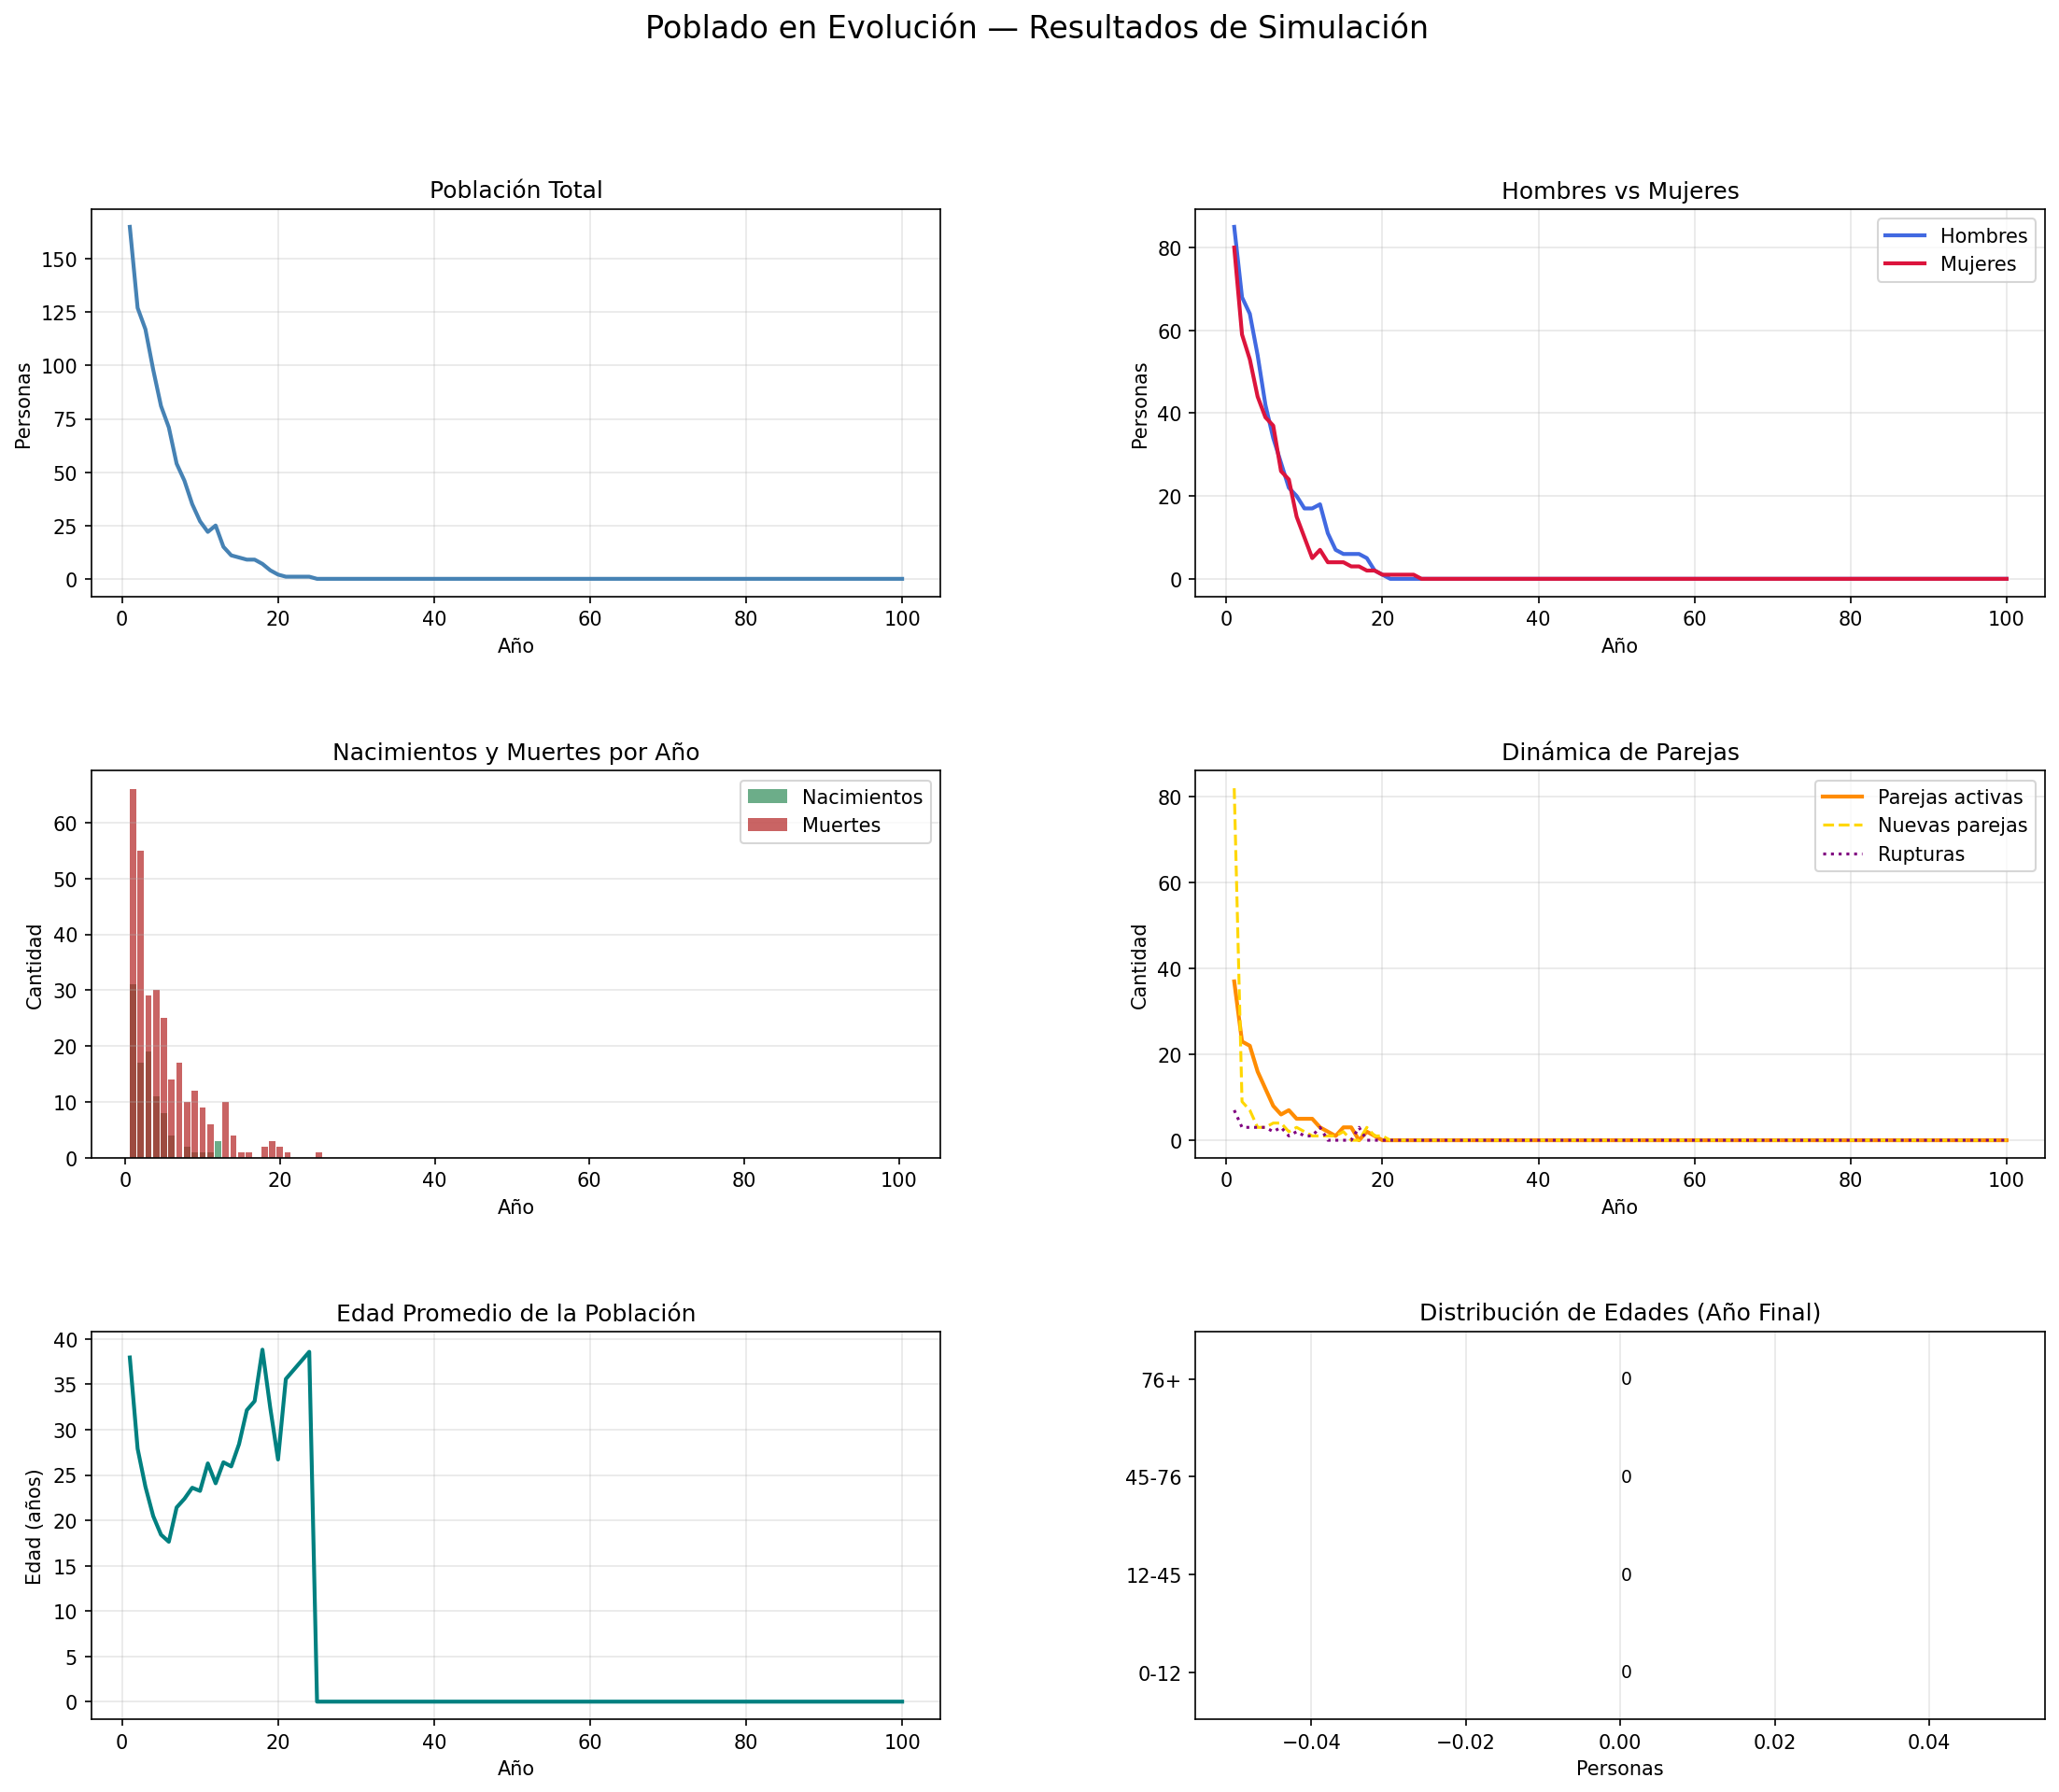
\includegraphics[width=\textwidth]{figures/E1_100x100.png}
  \caption{Experimento E1: 100~mujeres + 100~hombres, semilla~0.}
  \label{fig:e1}
\end{figure}

\begin{figure}[H]
  \centering
  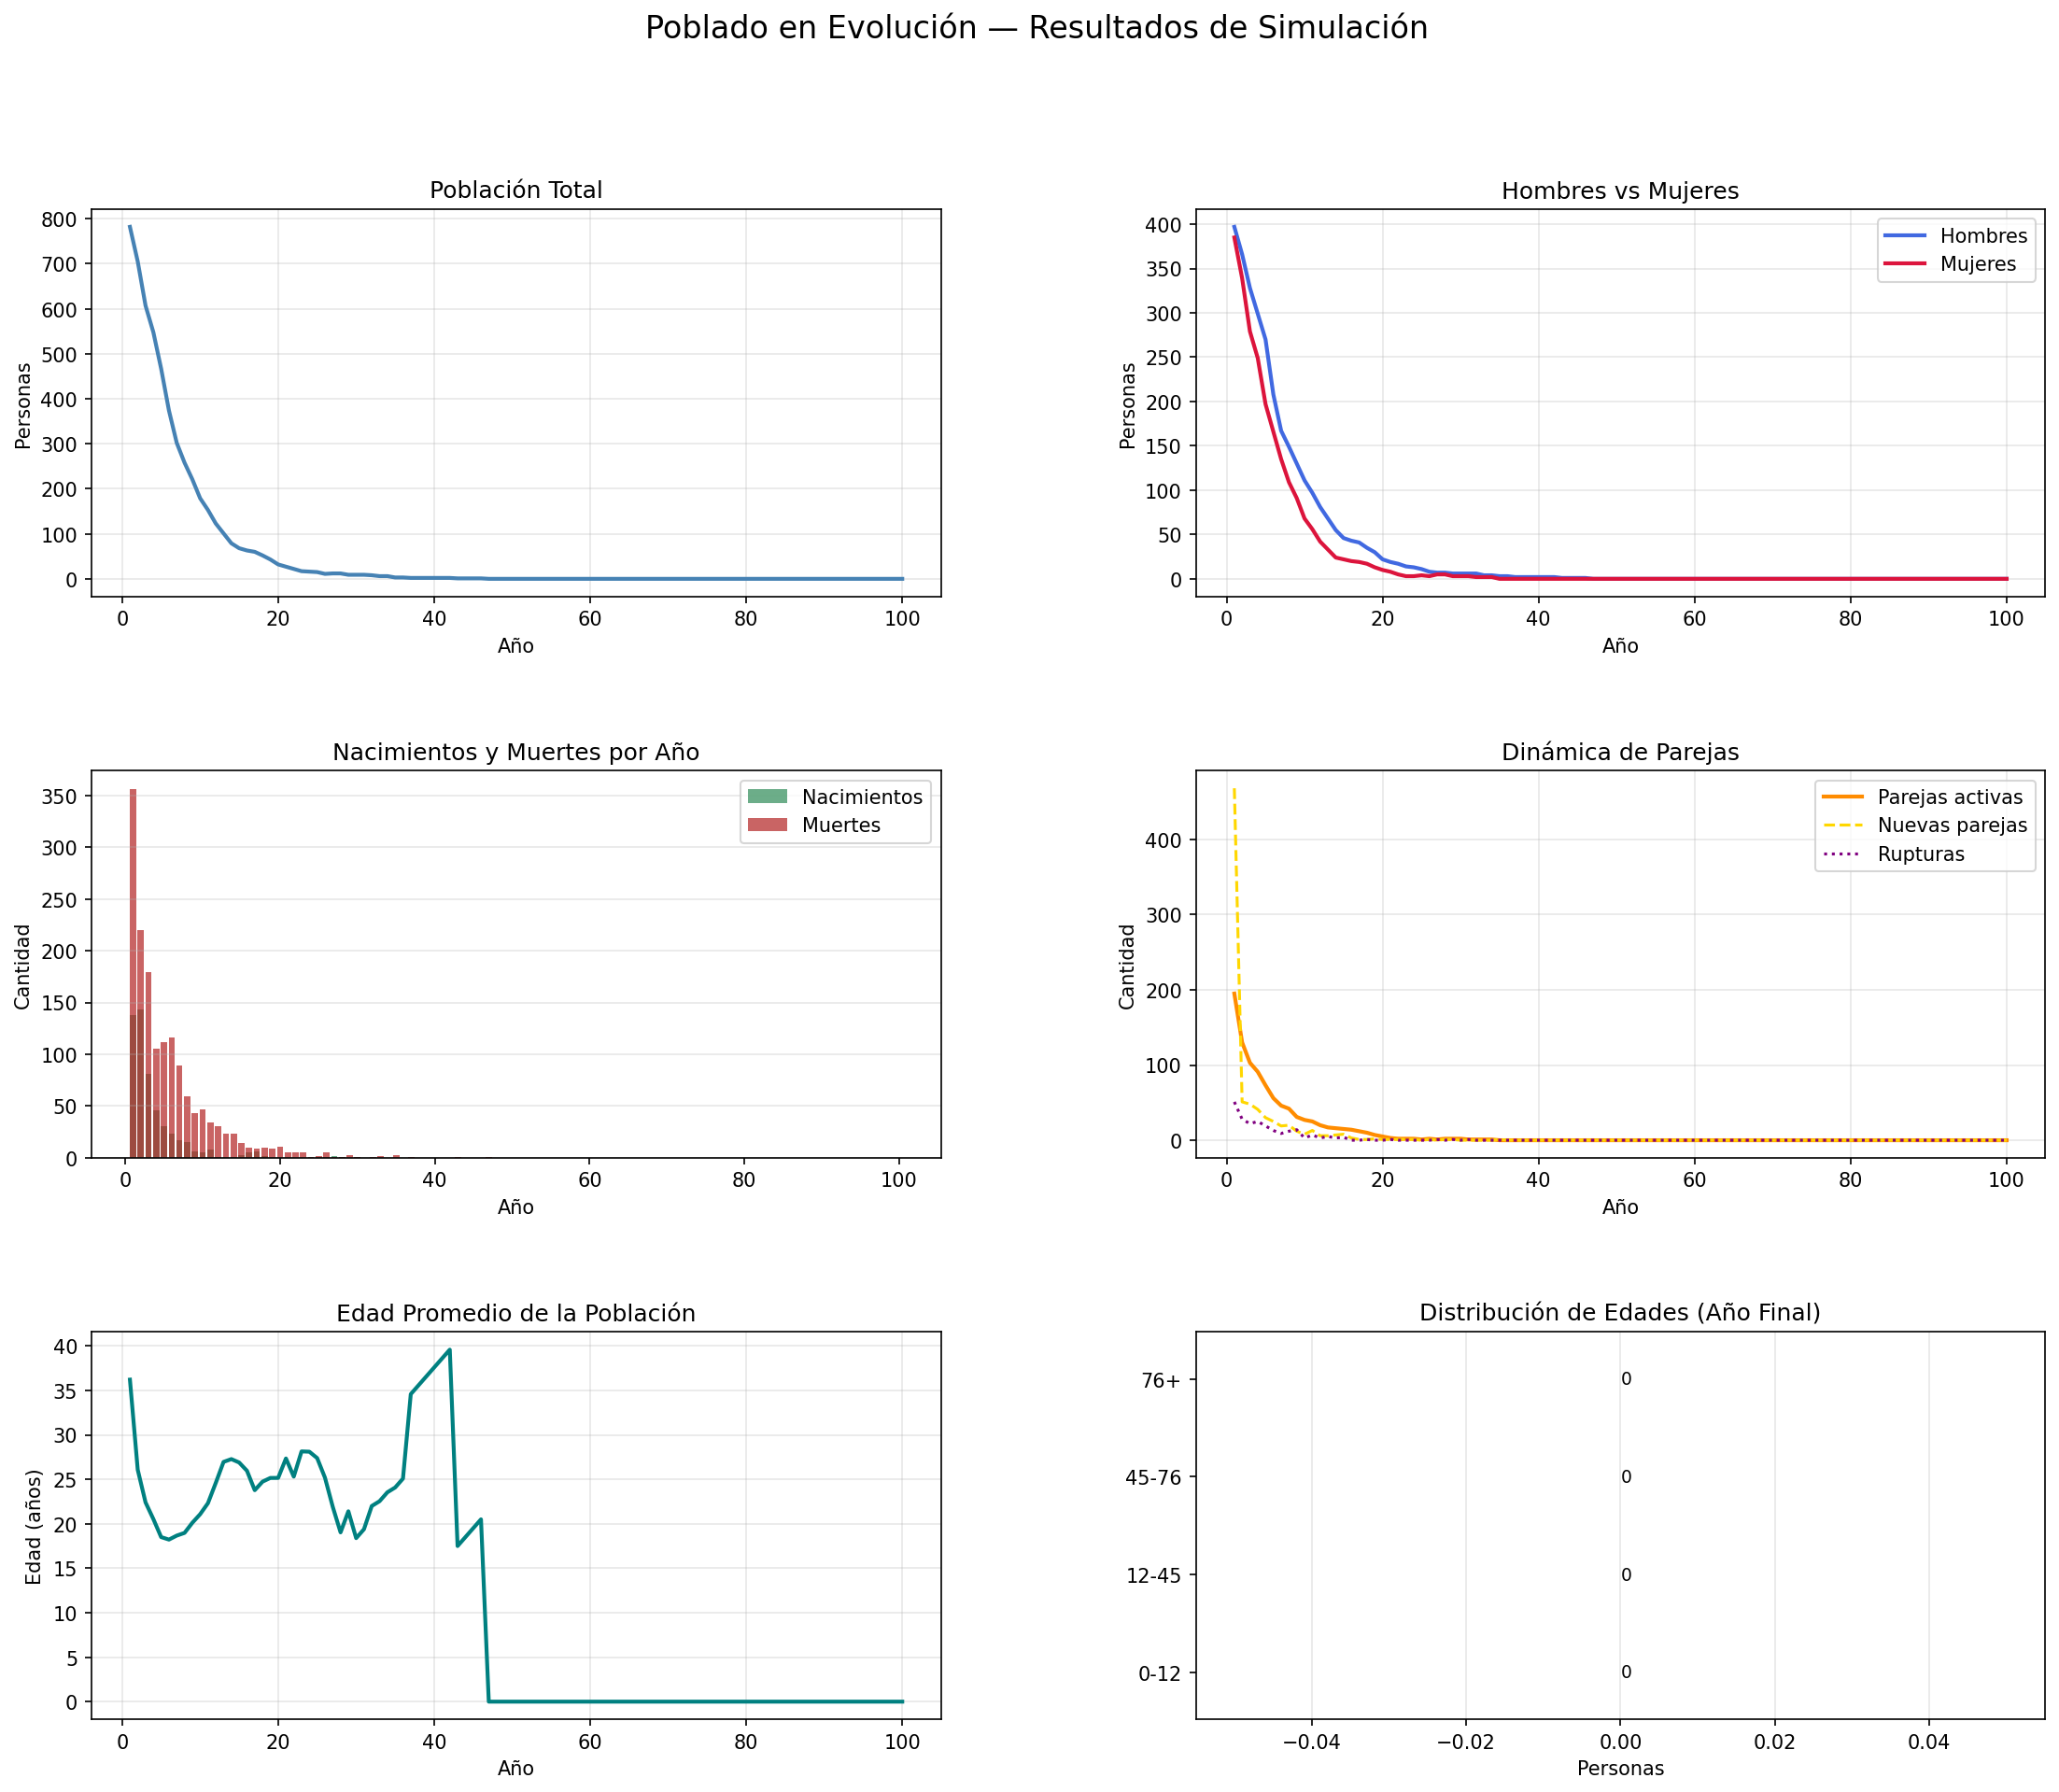
\includegraphics[width=\textwidth]{figures/E2_500x500.png}
  \caption{Experimento E2: 500~mujeres + 500~hombres, semilla~42.}
  \label{fig:e2}
\end{figure}

\begin{figure}[H]
  \centering
  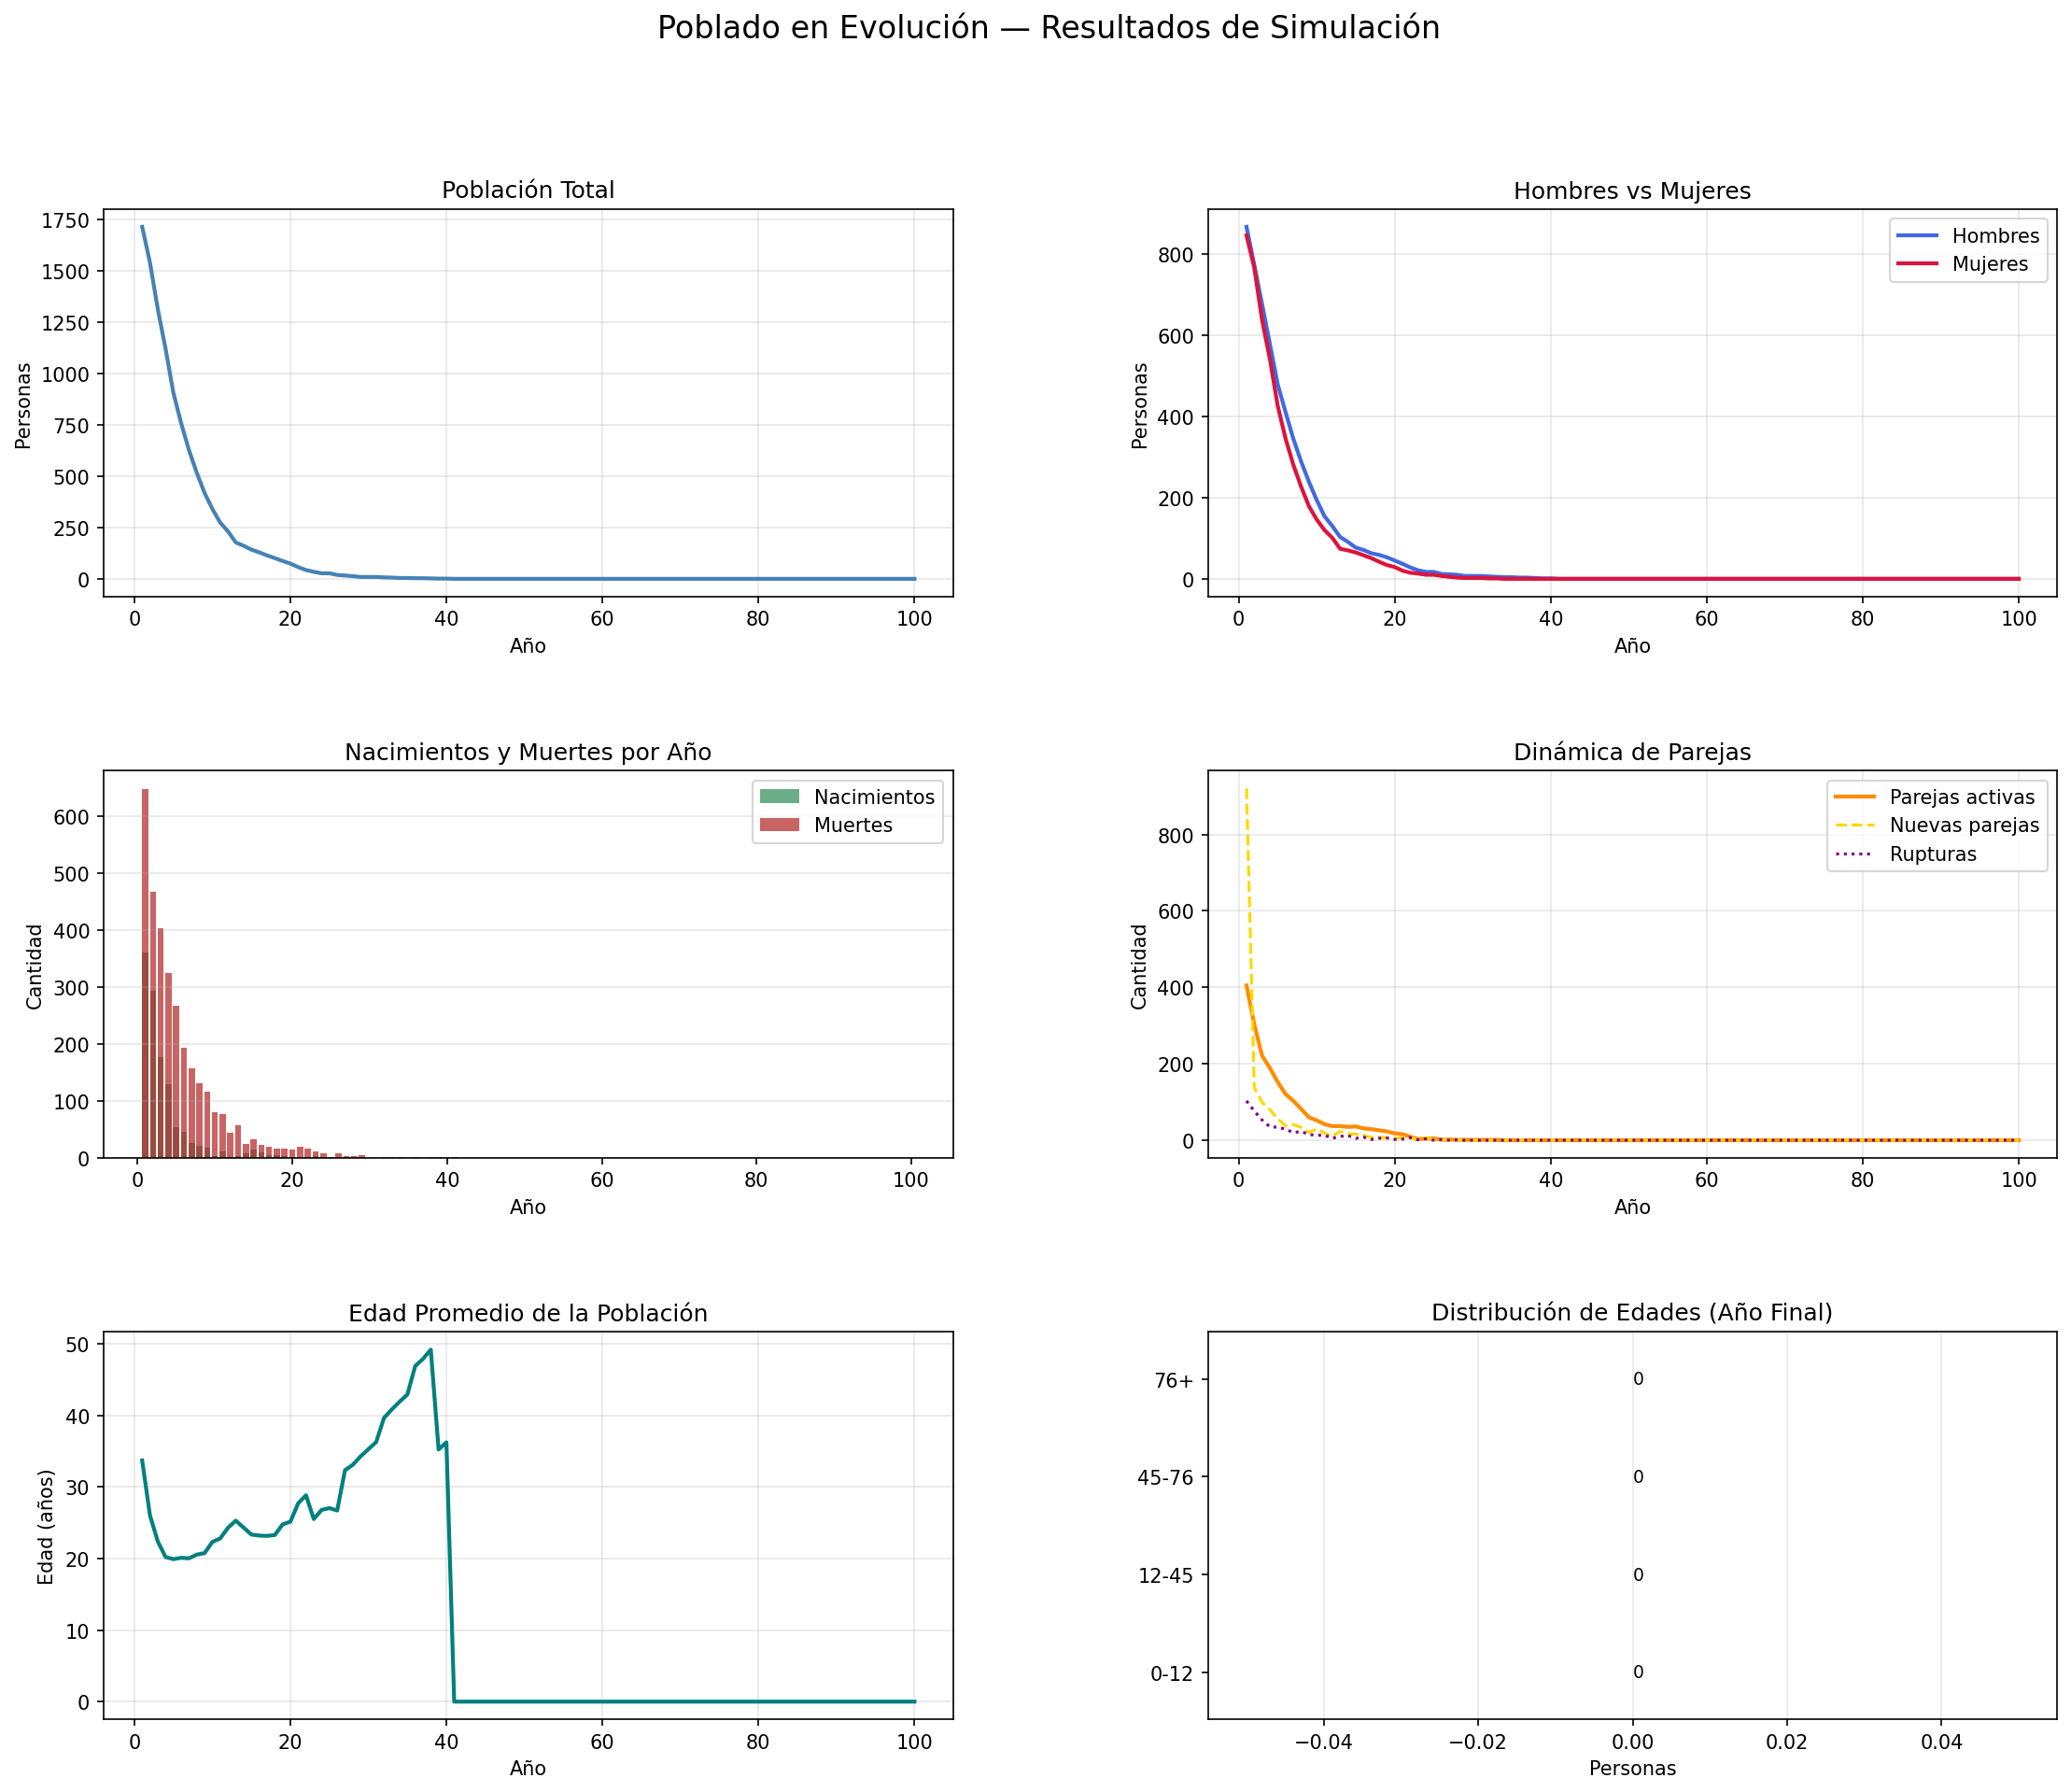
\includegraphics[width=\textwidth]{figures/E3_1000x1000.png}
  \caption{Experimento E3: 1000~mujeres + 1000~hombres, semilla~7.}
  \label{fig:e3}
\end{figure}

\subsection{Comparación de Interpretaciones de Embarazo}
\label{sec:comp_embarazo}

El mismo escenario E2 bajo los tres modos de embarazo
(Tabla~\ref{tab:comp_embarazo}) cuantifica el impacto semántico.
La diferencia entre modos no es cuantitativa sino cualitativa: producen
regímenes demográficos distintos e incomparables entre sí.

\begin{table}[H]
\caption{Comparación por modo de embarazo
         (E2: 500+500, semilla~42, mortalidad mensual, 100~años).}
\label{tab:comp_embarazo}
\centering
\small
\begin{tabular}{lrrrrrr}
\toprule
\textbf{Modo} & \textbf{Pob.\ final} & \textbf{Nacidos} &
\textbf{Muertos} & \textbf{TBN\,‰} & \textbf{TBM\,‰} &
\textbf{Crecim.\ nat.\,‰} \\
\midrule
\texttt{range}   &    896 &  1\,361 &  1\,465 & 12{,}8 & 15{,}5 & $-$2{,}7 \\
\texttt{annual}  & 14\,847 & 21\,186 &  7\,339 & 38{,}8 & 13{,}4 & $+$25{,}4 \\
\texttt{monthly} & 58\,266 & 79\,729 & 22\,463 & 48{,}7 & 13{,}9 & $+$34{,}8 \\
\bottomrule
\end{tabular}
\end{table}

La relación entre los tres resultados finales
(896\;:\;14\,847\;:\;58\,266) ilustra que la misma tabla de parámetros
puede producir comunidades que decrecen lentamente, que se multiplican por~15,
o que se multiplican por~58.
La interpretación semántica de $p$ es, en este modelo, el factor dominante
de la dinámica: más influyente que el tamaño poblacional inicial o que la
distribución de edades.

\begin{itemize}
  \item \textbf{\texttt{range}} produce crecimiento natural negativo
        ($-2{,}7$\,‰): la población decrece lentamente y envejece
        (edad media 60~años al final).

  \item \textbf{\texttt{annual}} produce crecimiento sostenido
        ($+25{,}4$\,‰, $\approx 2{,}5\,\%$ anual), comparable a tasas de
        países de alta fecundidad (Senegal, $\approx 35$\,‰).
        La población crece de 1\,000 a casi 15\,000 en un siglo.

  \item \textbf{\texttt{monthly}} produce crecimiento explosivo
        ($+34{,}8$\,‰, $\approx 3{,}5\,\%$ anual), por encima de las
        tasas históricas más altas jamás registradas.
        La población se multiplica por~58 en un siglo.
\end{itemize}

\subsection{Comparación de Frecuencia de Evaluación de Mortalidad}

La Tabla~\ref{tab:comp_muerte} compara los modos mensual y anual (S1b)
manteniendo constante el embarazo \texttt{range}.

\begin{table}[H]
\caption{Comparación de frecuencia de evaluación de mortalidad
         (E2: 500+500, semilla~42, embarazo \texttt{range}).}
\label{tab:comp_muerte}
\centering
\begin{tabular}{lrrrr}
\toprule
\textbf{Evaluación} & \textbf{Pob.\ final} & \textbf{Nacidos} &
\textbf{Muertos} & \textbf{Edad media final} \\
\midrule
Mensual (12/año) & 896 & 1\,361 & 1\,465 & 60{,}2~años \\
Anual (1/año)    & 984 & 1\,419 & 1\,435 & 55{,}9~años \\
\bottomrule
\end{tabular}
\end{table}

La diferencia ($\approx 10\,\%$ más supervivientes en modo anual) responde
a un mecanismo sutil: con evaluación anual, los individuos que morirían a
mediados de año sobreviven hasta el sorteo anual, participando en
emparejamientos y embarazos intermedios.
Ambos modos son matemáticamente equivalentes en esperanza sobre trayectorias
largas, pero la resolución temporal afecta las oportunidades reproductivas
mes a mes, produciendo una diferencia sistemática aunque pequeña.

\subsection{Réplicas e Intervalos de Confianza al 95\,\%}

Para cuantificar la incertidumbre de los resultados se ejecutaron
30~réplicas del escenario~E2 (Tabla~\ref{tab:replicas}).

\begin{table}[H]
\caption{Intervalos de confianza al 95\,\% para E2 (30~réplicas,
         motor \texttt{step}).}
\label{tab:replicas}
\centering
\begin{tabular}{lrl}
\toprule
\textbf{Métrica} & \textbf{Media} & \textbf{IC 95\,\%} \\
\midrule
Población final       & 913{,}5 & $[873{,}0,\; 954{,}1]$ \\
Tasa de supervivencia & 100\,\% & --- \\
\bottomrule
\end{tabular}
\end{table}

No hubo extinción en ninguna de las 30~corridas, por lo que la incertidumbre
se reporta sobre la población final.
El IC estrecho ($\pm 41$ sobre una media de 913) indica resultados
estadísticamente estables.
El número mínimo de réplicas recomendado por la fórmula de $n_{\min}$ para
un error relativo del 5\,\% es consistente con las 30~réplicas ejecutadas.

\subsection{Prueba de Hipótesis: Distribución de Edades Iniciales}
\label{sec:hipotesis}

Se compara el año de extinción bajo dos distribuciones de edades iniciales:
$U(0,100)$ (adversa) y $U(0,40)$ (más joven), con 1\,000~individuos y
15~réplicas cada una.
La hipótesis nula es igualdad de medias:
\[
  H_0: \mu_{U(0,100)} = \mu_{U(0,40)}, \qquad
  H_1: \mu_{U(0,100)} \ne \mu_{U(0,40)}.
\]

\begin{table}[H]
\caption{Prueba $t$ de Welch: $U(0,100)$ vs $U(0,40)$ (15~réplicas cada uno).}
\label{tab:hipotesis}
\centering
\begin{tabular}{lrrrrl}
\toprule
\textbf{Comparación} & $\bar{X}_1$ & $\bar{X}_2$ & $t$ &
\textbf{V.C.\ ($\alpha{=}0{,}05$)} & \textbf{Decisión} \\
\midrule
$U(0,100)$ vs $U(0,40)$ & 45{,}3 & 49{,}0 & $-1{,}45$ & 2{,}060 & No rechazar $H_0$ \\
\bottomrule
\end{tabular}
\end{table}

Con $|t| = 1{,}45 < 2{,}06$ no se rechaza $H_0$ al 5\,\%.
La diferencia de $\approx 4$~años en el año de extinción no es
estadísticamente significativa con 15~réplicas, aunque la dirección es la
esperada: $U(0,40)$ produce poblaciones más jóvenes y con mayor resistencia.
Para detectar esta diferencia con potencia adecuada se requeriría un número
mayor de réplicas, calculable mediante la fórmula de $n_{\min}$.

% ──────────────────────────────────────────────────────────────────────────
\section{Rigor Metodológico: Calendario de Eventos Discretos}
\label{sec:fel}
% ──────────────────────────────────────────────────────────────────────────

\subsection{Motivación: del Paso Fijo al Evento con Timestamp}

El motor \texttt{step} es correcto y suficiente para obtener resultados
demográficos válidos.
Sin embargo, desde el punto de vista de la teoría de DES, tiene una
limitación conceptual: los eventos no tienen un instante preciso dentro
del mes en que ocurren.
Si una persona muere y otra forma pareja en el mismo mes, el simulador no
puede establecer cuál ocurrió antes: el orden está codificado en el bucle,
no derivado de los timestamps de los eventos.

Un simulador de eventos discretos clásico~\cite{banks2001} resuelve esto
con una \textbf{Future Event List} (FEL): cada evento tiene un timestamp
$\tau$ y se procesa en orden cronológico estricto (\emph{next-event
paradigm}).
Esto hace explícita la regla ``procesa el evento más temprano primero'',
separa el \emph{qué} del \emph{cuándo} de cada transición, y facilita
extender el modelo con eventos diferidos sin reestructurar el motor.

La pregunta que responde esta sección es metodológicamente relevante:
\textbf{¿cambian los resultados demográficos cuando adoptamos la
formulación FEL más rigurosa?}
Si ambos motores producen resultados estadísticamente consistentes, el
modelo está bien definido y es robusto a la elección de implementación.

\subsection{Arquitectura del Motor FEL (\texttt{calendar\_strong})}

El motor \texttt{calendar\_strong\_simulator.py} implementa una cola de
prioridad (\texttt{heapq}) donde cada evento es una estructura:
\begin{center}
\texttt{(month, priority, seq, kind, a, b)}
\end{center}
El campo \texttt{month} es el timestamp entero en meses;
\texttt{priority} es una prioridad causal intra-mes que reproduce el orden
correcto de fases (envejecimiento antes de muertes, etc.);
\texttt{seq} desempata eventos del mismo instante y prioridad.

Cada fase mensual ---envejecimiento, muertes, rupturas, emparejamientos,
embarazos, nacimientos--- se programa como un evento con su timestamp
correspondiente, ejecutándose en orden cronológico explícito.
Los eventos obsoletos (p.~ej., nacimientos de personas que han muerto)
se detectan y descartan al ser procesados.

Esta formulación hace posible insertar en el futuro eventos diferidos con
timestamps arbitrarios (migraciones, intervenciones sanitarias, shocks
demográficos puntuales) sin reestructurar el motor ni modificar el bucle
principal.

\subsection{Comparación Empírica: \texttt{step} vs \texttt{calendar\_strong}}

La Tabla~\ref{tab:step_vs_strong} compara ambos motores bajo la misma
configuración (500+500, 50~años, mortalidad mensual, embarazo \texttt{range},
semillas~0--9).

\begin{table}[H]
\caption{Comparación empírica entre motor clásico y FEL fuerte
         (promedios de 10~réplicas, 50~años).}
\label{tab:step_vs_strong}
\centering
\begin{tabular}{lrr}
\toprule
\textbf{Métrica} & \textbf{\texttt{step}} & \textbf{\texttt{calendar\_strong}} \\
\midrule
Población final media        & 965{,}9 & 976{,}8 \\
Población final (mín--máx)   & 888--1039 & 919--1044 \\
Nacidos totales (media)      & 685{,}5 & 697{,}4 \\
Muertos totales (media)      & 719{,}6 & 720{,}6 \\
Edad media final (años)      & 57{,}29 & 55{,}89 \\
Supervivencia al año~50      & 100\,\% & 100\,\% \\
Tiempo medio por corrida (s) & 1{,}13 & 1{,}68 \\
\bottomrule
\end{tabular}
\end{table}

Los dos motores producen resultados del mismo orden de magnitud con
tendencias cualitativas idénticas.
La diferencia en población final media ($\approx 1{,}1\,\%$) es sistemática
pero menor que la variabilidad entre semillas: en el paradigma next-event,
ciertos emparejamientos y embarazos que en \texttt{step} quedarían
desplazados al mes siguiente se procesan en el instante correcto, preservando
oportunidades reproductivas en ventanas temporales más finas.
El costo computacional de \texttt{calendar\_strong} es $\approx 1{,}5\times$
mayor por el overhead de gestionar la FEL (inserciones y extracciones de la
cola de prioridad).

\paragraph{Ventajas de cada enfoque.}
\begin{itemize}
  \item \texttt{step}: más simple de leer, depurar y explicar; óptimo para
        experimentación rápida y docencia.
  \item \texttt{calendar\_strong}: metodológicamente alineado con DES
        clásico; óptimo para extensibilidad con eventos diferidos complejos.
\end{itemize}

\subsection{Análisis Monte Carlo: Motores e Interpretaciones}
\label{sec:mc}

Para confirmar que las conclusiones no dependen de semillas particulares,
se realizó un análisis Monte Carlo cruzando motores y modos de embarazo,
usando 6~semillas por combinación (Tabla~\ref{tab:mc}).

\begin{table}[H]
\caption{Resumen Monte Carlo cruzado: motores $\times$ interpretaciones
         (200+200, 20~años, mortalidad mensual, 6~réplicas).}
\label{tab:mc}
\centering
\small
\begin{tabular}{llrrrr}
\toprule
\textbf{Motor} & \textbf{Embarazo} & \textbf{Pob.\ media} &
\textbf{Desv.\ est.} & \textbf{Nacidos med.} & \textbf{Muertos med.} \\
\midrule
\texttt{step}             & \texttt{range}   & 397{,}8 & 25{,}8 & 117{,}2 & 119{,}3 \\
\texttt{step}             & \texttt{annual}  & 747{,}0 & 29{,}8 & 542{,}7 & 195{,}7 \\
\texttt{step}             & \texttt{monthly} & 1434{,}0 & 46{,}9 & 1357{,}5 & 323{,}5 \\
\texttt{calendar\_strong} & \texttt{range}   & 403{,}3 & 20{,}6 & 121{,}5 & 118{,}2 \\
\texttt{calendar\_strong} & \texttt{annual}  & 744{,}3 & 39{,}8 & 535{,}7 & 191{,}3 \\
\texttt{calendar\_strong} & \texttt{monthly} & 1428{,}7 & 27{,}7 & 1331{,}7 & 303{,}0 \\
\bottomrule
\end{tabular}
\end{table}

Los datos confirman tres hallazgos estructurales:

\begin{enumerate}
  \item \textbf{La interpretación de embarazo es el factor dominante.}
        Entre \texttt{range} y \texttt{monthly} hay un factor
        $\approx 3{,}6\times$ en población final, frente a $\approx 1{,}4\,\%$
        entre motores para igual interpretación.
        El orden \texttt{range} $<$ \texttt{annual} $<$ \texttt{monthly}
        es robusto a través de todas las semillas y ambos motores.

  \item \textbf{Los dos motores son estadísticamente consistentes.}
        Para igual modo de embarazo, la diferencia entre motores es menor
        que la desviación estándar intra-motor.
        Esto valida que ambas implementaciones modelan esencialmente el
        mismo proceso demográfico.

  \item \textbf{El análisis multi-semilla es necesario.}
        La desviación estándar de la población final es del orden del
        5--7\,\% de la media; comparar una sola semilla puede inducir
        conclusiones erróneas.
        El análisis Monte Carlo produce estimaciones más estables y
        cuantifica la variabilidad natural del proceso.
\end{enumerate}

\subsection{Análisis Genealógico por Configuración}
\label{sec:genealogy}

El módulo \texttt{sim/genealogy.py} construye un grafo dirigido
(\texttt{networkx}, \texttt{DiGraph}) sobre el conjunto completo de personas
del simulador.
Cada nodo es un individuo con atributos (sexo, año de nacimiento, estado
vital, número de hijos); cada arista es una relación padre/madre
$\rightarrow$ hijo.
El grafo se puede exportar en formato GEXF para análisis externo con Gephi.

Las métricas clave del árbol genealógico son: número de nodos y aristas,
número máximo de generaciones (profundidad del grafo desde fundadores),
número de fundadores sin descendencia, y tamaño del mayor subgrafo conexo.

Estas métricas revelan la arquitectura reproductiva subyacente a cada
configuración de forma cualitativa y complementaria a los indicadores
demográficos agregados:

\begin{itemize}
  \item \textbf{Bajo \texttt{range}}, los árboles son \textbf{anchos y
        superficiales}.
        La baja tasa mensual de embarazo produce 3--4~generaciones en
        100~años.
        La mayoría de los fundadores iniciales no deja descendencia en la
        simulación: fallecieron antes de tener hijos, o sus hijos murieron
        sin reproducirse.
        El mayor subgrafo conexo representa una fracción pequeña del total.
        Este patrón describe una demografía estancada donde la reproducción
        es insuficiente para construir linajes largos.

  \item \textbf{Bajo \texttt{annual}}, los árboles son
        \textbf{moderadamente profundos y conectados}.
        Emergen 6--7~generaciones.
        Más de la mitad de los fundadores tiene al menos un descendiente.
        Se observan familias extensas con ramificaciones claras, y el mayor
        subgrafo conexo cubre una proporción significativa de la población.

  \item \textbf{Bajo \texttt{monthly}}, los árboles se convierten en
        \textbf{redes densas}.
        Pueden emerger más de 10~generaciones en un siglo, prácticamente
        todos los fundadores tienen múltiples descendientes, y el grafo
        tiende a un único componente gigante donde casi todos los individuos
        están relacionados por algún camino.
        El árbol del fundador más prolífico puede abarcar miles de nodos.
\end{itemize}

La comparación entre motores (\texttt{step} vs \texttt{calendar\_strong})
para igual interpretación muestra estructuras genealógicas estadísticamente
equivalentes: las diferencias en número de generaciones y porcentaje de
fundadores con descendencia no son significativas entre motores.
Esto confirma que ambos implementan el mismo proceso reproductivo subyacente,
y que las pequeñas diferencias en población final no alteran la arquitectura
familiar emergente.

El árbol genealógico sirve así como \textbf{herramienta de diagnóstico
cualitativo}: mientras las tablas de resultados muestran cuántas personas
viven, el grafo muestra \emph{qué estructura familiar} produjo ese número,
completando la imagen de la dinámica demográfica.

% ──────────────────────────────────────────────────────────────────────────
\clearpage
\section{Implementación}
\label{sec:implementacion}
% ──────────────────────────────────────────────────────────────────────────

\subsection{Arquitectura de Módulos}

El proyecto se organiza en los módulos de la Tabla~\ref{tab:modules}.

\begin{table}[H]
\caption{Módulos del proyecto y sus responsabilidades.}
\label{tab:modules}
\centering
\begin{tabular}{ll}
\toprule
\textbf{Módulo} & \textbf{Responsabilidad} \\
\midrule
\texttt{sim/tables.py}      & Tablas de probabilidad del enunciado y funciones de lookup \\
\texttt{sim/random\_vars.py} & Generador LCG y distribuciones derivadas \\
\texttt{sim/stats\_tools.py} & $\chi^2$, KS, IC, $t$ de Welch, $n_{\min}$ \\
\texttt{sim/person.py}      & Entidad Persona \\
\texttt{sim/couple.py}      & Entidad Pareja \\
\texttt{sim/simulator.py}   & Motor de paso mensual (\texttt{step}) \\
\texttt{sim/calendar\_strong\_simulator.py} & Motor FEL (\texttt{calendar\_strong}) \\
\texttt{sim/factory.py}     & Selector de motor \\
\texttt{sim/monte\_carlo.py} & Runner de $N$ réplicas con agregación estadística \\
\texttt{sim/sensitivity.py} & Análisis de sensibilidad y prueba de Welch \\
\texttt{sim/genealogy.py}   & Árbol genealógico (\texttt{networkx}) \\
\texttt{main.py}            & Punto de entrada CLI \\
\texttt{visualize.py}       & Gráficas (\texttt{matplotlib}) \\
\texttt{app.py}             & Dashboard interactivo (Streamlit) \\
\bottomrule
\end{tabular}
\end{table}

\subsection{Diagrama de Flujo del Bucle Mensual}

\begin{figure}[H]
\centering
\fbox{\parbox{0.85\textwidth}{%
\centering
\vspace{0.3cm}
\textbf{Inicio del mes $t$}\\[4pt]
$\downarrow$\\[2pt]
Envejecer a todos (+1 mes)\\[2pt]
$\downarrow$\\[2pt]
Evaluar muertes (Bernoulli por persona)\\[2pt]
$\downarrow$\\[2pt]
Evaluar rupturas (Bernoulli por pareja)\\[2pt]
$\downarrow$\\[2pt]
Decrementar contadores de soledad\\[2pt]
$\downarrow$\\[2pt]
Intentar formación de parejas (shuffle + iteración)\\[2pt]
$\downarrow$\\[2pt]
Evaluar embarazos (Bernoulli por mujer)\\[2pt]
$\downarrow$\\[2pt]
Procesar nacimientos (gestación completada)\\[2pt]
$\downarrow$\\[2pt]
\textbf{Fin del mes $t$} (registrar si $t \bmod 12 = 0$)
\vspace{0.3cm}
}}
\caption{Flujo de procesamiento en cada paso mensual del motor \texttt{step}.}
\label{fig:flujo}
\end{figure}

\subsection{Complejidad Computacional}

El costo dominante por mes es el emparejamiento: $O(n_H \cdot n_M)$ en el
peor caso, pero $O(\min(n_H, n_M))$ en la práctica con el barajado
secuencial (S7), porque la mayoría de intentos termina en la primera pareja
compatible.
Los demás eventos son $O(n)$ donde $n$ es la población total.
El motor \texttt{calendar\_strong} añade $O(k \log k)$ por las operaciones
sobre la FEL, donde $k$ es el número de eventos en cola ($\approx 7n$
en el peor caso por fase mensual).

\subsection{Dashboard Interactivo}

La aplicación \texttt{app.py} (Streamlit) permite explorar la simulación
en tiempo real: ajustar motor, interpretaciones, tamaño de población,
semilla y horizonte, con actualización inmediata de gráficas y métricas
estadísticas.
Sirve como herramienta de comunicación de resultados y como entorno de
experimentación rápida ante nuevas hipótesis.

Para lanzar el dashboard, basta ejecutar desde la raíz del proyecto:

\begin{lstlisting}[language=bash, numbers=none]
streamlit run app.py
\end{lstlisting}

Streamlit abre automáticamente el navegador en \texttt{http://localhost:8501}.
Todos los parámetros son ajustables desde la barra lateral sin necesidad de
modificar el código: motor de simulación, semilla, tamaño de la población
inicial, horizonte temporal e interpretación de probabilidades.
La Figura~\ref{fig:dashboard} muestra la interfaz con una ejecución de ejemplo.

\begin{figure}[H]
  \centering
  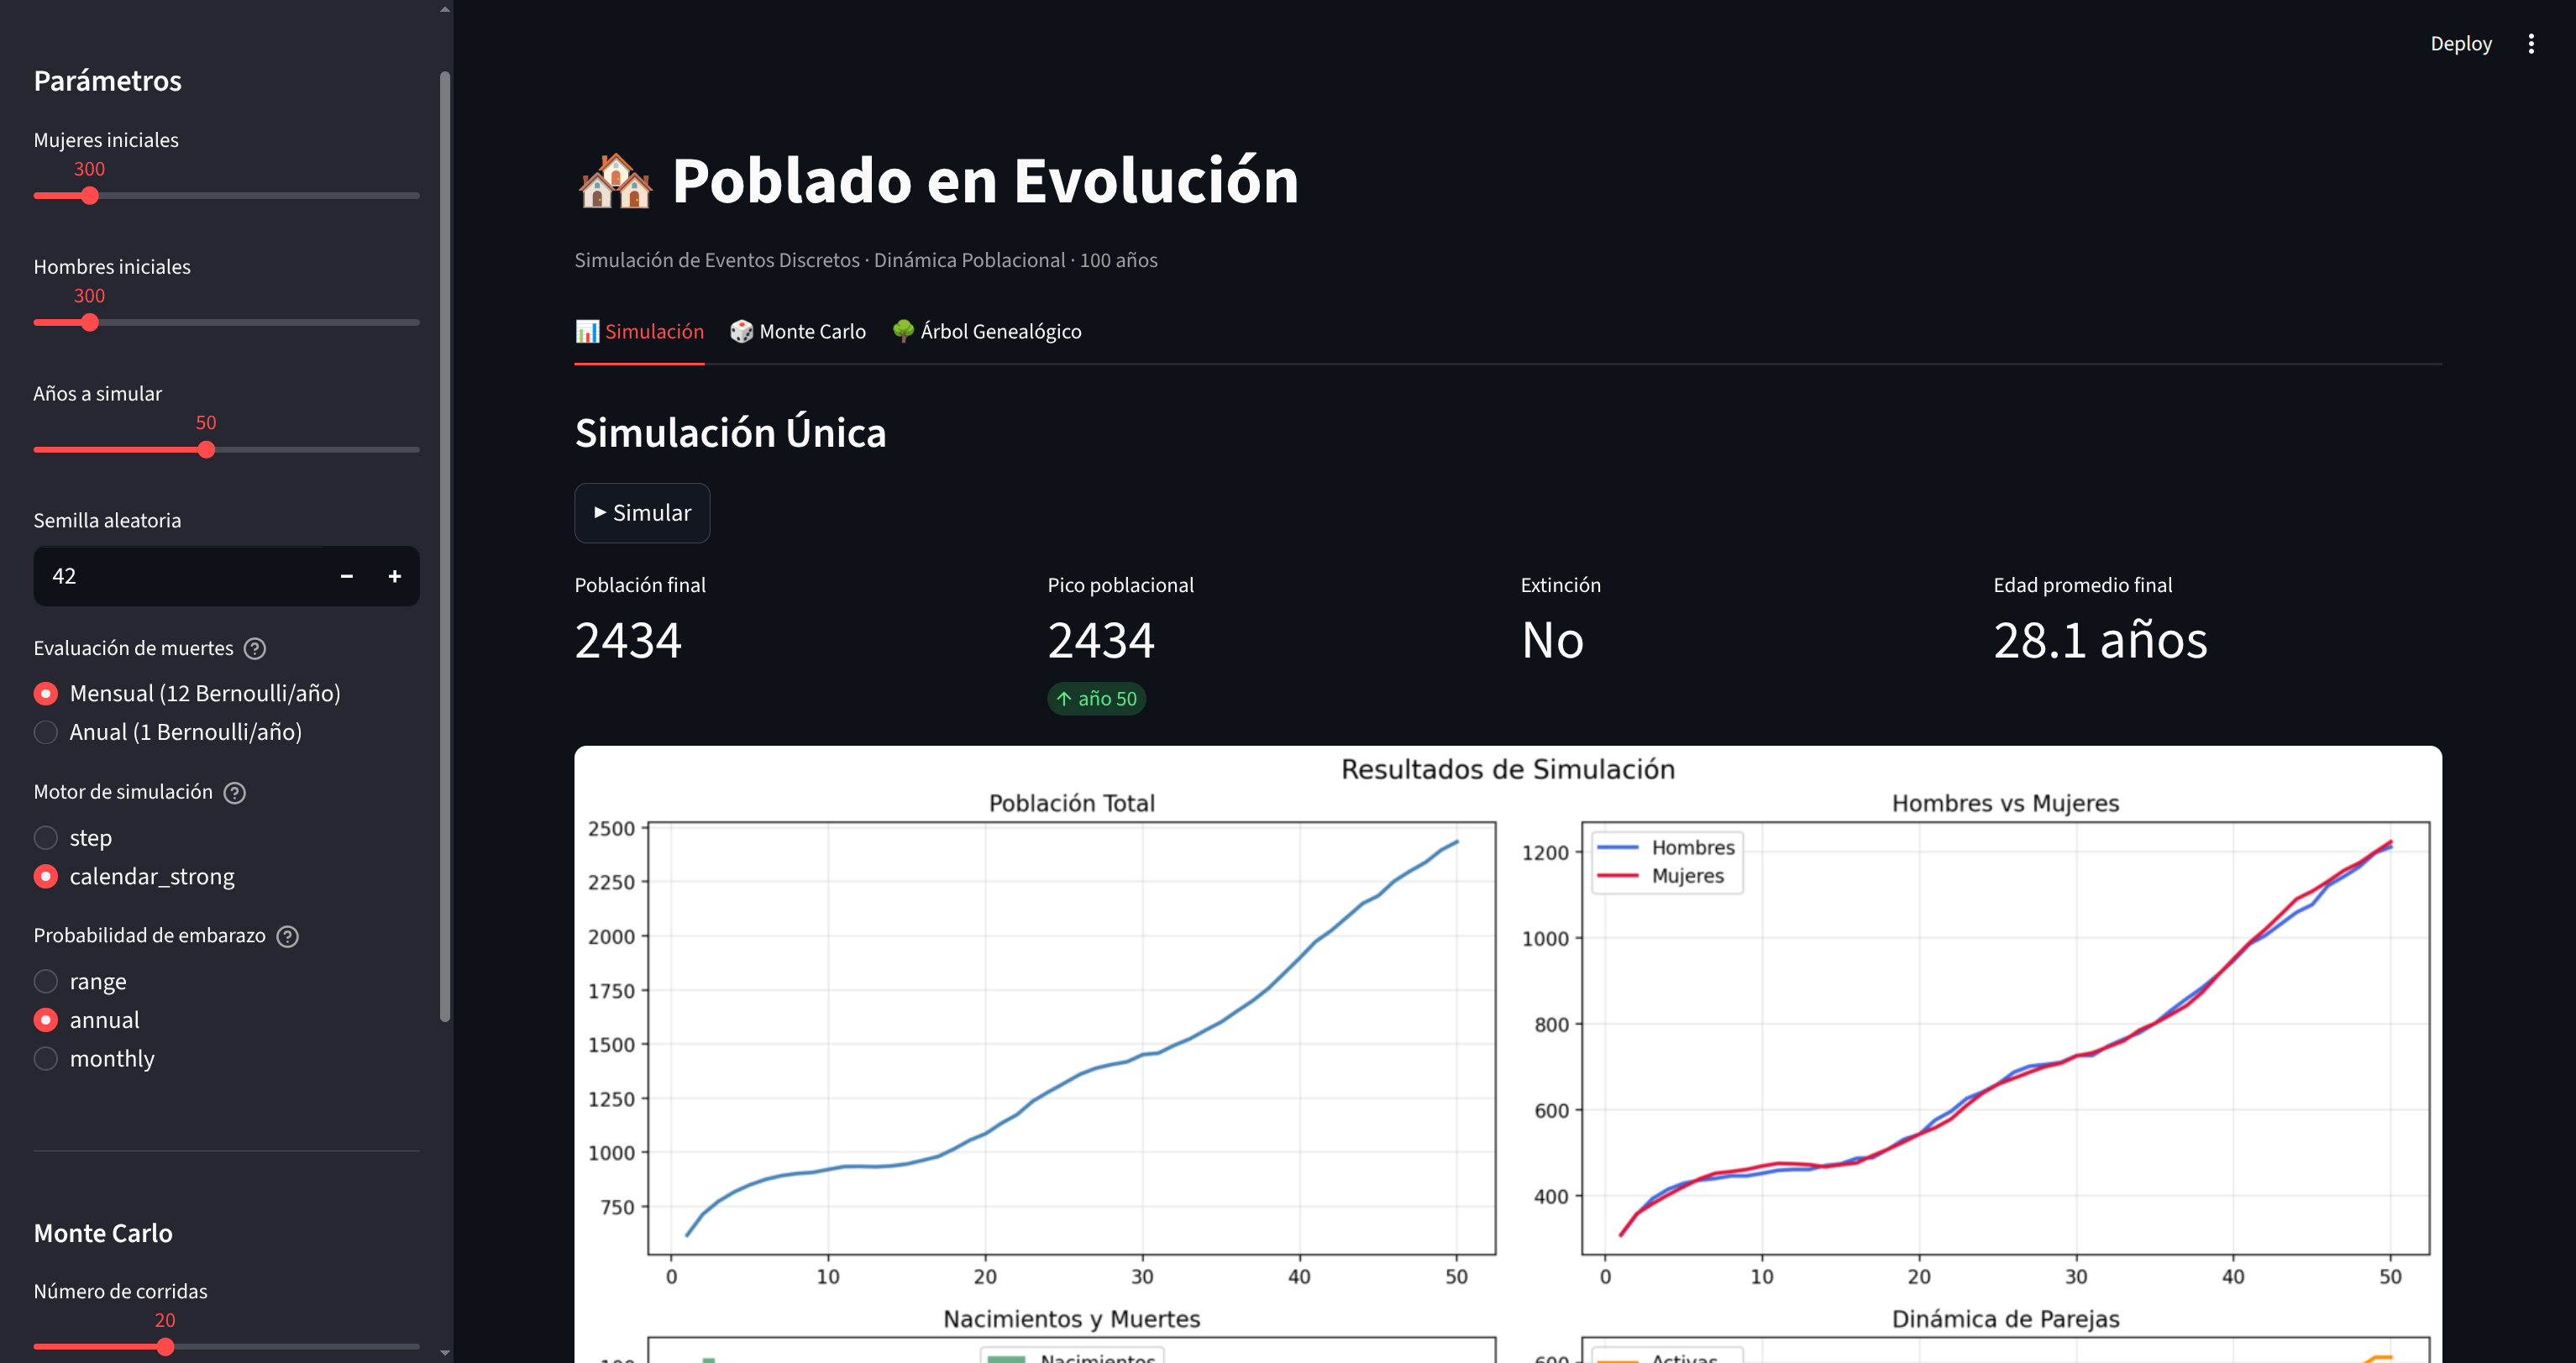
\includegraphics[width=\textwidth]{figures/dashboard.png}
  \caption{Dashboard interactivo de \texttt{app.py}. La barra lateral controla
           los parámetros de la simulación; el área principal muestra
           evolución poblacional, distribución etaria, formación de parejas
           y métricas estadísticas en tiempo real.}
  \label{fig:dashboard}
\end{figure}

% ──────────────────────────────────────────────────────────────────────────
\section{Conclusiones}
\label{sec:conclusiones}
% ──────────────────────────────────────────────────────────────────────────

El trabajo produjo tres contribuciones articuladas, cada una consecuencia
natural de la anterior.

\paragraph{1. Infraestructura estadística propia como fundamento.}
La construcción desde cero del LCG (con parámetros validados teórica y
empíricamente), las distribuciones derivadas y las herramientas estadísticas
establece una base de \textbf{reproducibilidad fuerte}: cualquier resultado
puede replicarse exactamente a partir de la semilla documentada.
Esta capa no es un requisito burocrático; es lo que hace posible la
comparación controlada entre interpretaciones y motores, porque cualquier
diferencia observada puede atribuirse a la variable que cambió, no a
aleatoriedad no gestionada.
La arquitectura de dos capas ---núcleo LCG + funciones de nivel superior---
garantiza que toda la aleatoriedad del sistema fluya por un único árbol
pseudoaleatorio auditabl.

\paragraph{2. La interpretación semántica como hallazgo central.}
La primera ejecución con la lectura más directa ($p$ = tasa mensual) produjo
una población biológicamente imposible de más de 40\,000~personas a partir
de 600~individuos, señalando inequívocamente que la interpretación era
incorrecta.
El análisis sistemático de las tres lecturas posibles mostró que la elección
entre interpretaciones no es una corrección técnica menor: produce diferencias
de un factor $65\times$ en población final
(58\,266 bajo \texttt{monthly} vs 896 bajo \texttt{range} para el mismo
escenario E2).

La interpretación de \textbf{probabilidad acumulada por rango}, coherente
entre mortalidad y fecundidad, produce la dinámica más plausible: declive
suave, envejecimiento progresivo, sin extinción en 100~años.
La lección metodológica es que una tabla de parámetros sin especificación
semántica explícita es ambigua, y esa ambigüedad puede dominar la dinámica
del modelo.
La respuesta correcta no es elegir arbitrariamente sino documentar cada
interpretación, cuantificar su efecto mediante el protocolo de expansión
controlada, y decidir con criterio justificado.

\paragraph{3. Validación cruzada mediante FEL y Monte Carlo.}
La introducción del motor \texttt{calendar\_strong} responde a una pregunta
metodológica precisa: ¿son los resultados artefactos del orden de
procesamiento del bucle mensual, o reflejan genuinamente el modelo
demográfico subyacente?
El análisis Monte Carlo sobre 6~réplicas $\times$ 2~motores $\times$
3~modos de embarazo confirma que los motores son estadísticamente
consistentes (diferencias menores que la desviación estándar intra-motor),
validando la robustez del modelo.
Las diferencias menores pero sistemáticas del motor FEL (ligera mayor
natalidad) son coherentes con su paradigma next-event, que preserva
oportunidades reproductivas en ventanas temporales más finas.

\paragraph{El árbol genealógico como diagnóstico cualitativo.}
Los árboles genealógicos revelan la arquitectura reproductiva emergente:
árboles superficiales con muchos fundadores sin descendencia bajo
\texttt{range} (demografía estancada, 3--4~generaciones en un siglo),
árboles moderadamente profundos bajo \texttt{annual} (6--7~generaciones,
familias extensas), y redes densas con más de 10~generaciones bajo
\texttt{monthly} (casi todos los individuos relacionados).
Para igual interpretación, los dos motores producen estructuras
genealógicas equivalentes, confirmando la consistencia a nivel cualitativo.
Este análisis complementa los indicadores agregados mostrando \emph{qué
estructura familiar} subyace a cada régimen demográfico.

\paragraph{Cambios interesantes observados.}
El tránsito entre interpretaciones no produce solo una escala diferente en
la población final: produce diferencias cualitativas en la pirámide de
edades (de 21{,}9~años a 52{,}5~años de edad media final para el mismo
escenario), en la dinámica de parejas y en la profundidad del árbol
genealógico.
En el análisis Monte Carlo, el modo \texttt{range} es el único con
crecimiento natural negativo; los otros dos tienen crecimiento positivo
sostenido.
Esta no-linealidad en la respuesta del modelo a la interpretación es el
hallazgo más importante: el modelo no es sensible a la interpretación,
es \emph{cualitativamente controlado} por ella.

\paragraph{Extensiones futuras.}
La arquitectura FEL permite insertar eventos diferidos con timestamps
arbitrarios sin modificar el motor: migración, enfermedades epidémicas,
variaciones estacionales de fertilidad o shocks demográficos puntuales.
La infraestructura estadística propia puede ampliarse con pruebas adicionales
(Anderson-Darling, CUSUM) sin dependencias externas.
Comparar la distribución inicial $U(0,100)$ con una pirámide etaria más
realista (p.~ej., triangular con moda en~0) permitiría separar el efecto de
la condición inicial adversa del efecto de las reglas demográficas.

% ──────────────────────────────────────────────────────────────────────────
\section*{Repositorio del Proyecto}

El código fuente completo, incluyendo la implementación de todas las
variables aleatorias, los experimentos y el dashboard interactivo, se
encuentra disponible en:

\begin{center}
  \url{https://github.com/perezcam/Sim-City}
\end{center}

% ──────────────────────────────────────────────────────────────────────────
\begin{thebibliography}{9}

\bibitem{axtell2000}
Axtell, R., Epstein, J.M.: Agent-Based Modeling: Understanding Our Creations.
Bulletin of the Santa Fe Institute \textbf{14}, 28--32 (2000)

\bibitem{banks2001}
Banks, J., Carson, J.S., Nelson, B.L., Nicol, D.M.:
Discrete-Event System Simulation, 3rd edn.
Prentice-Hall, Upper Saddle River (2001)

\bibitem{kelton2015}
Kelton, W.D., Smith, J.S., Sturrock, D.T.:
Simio and Simulation: Modeling, Analysis, Applications, 3rd edn.
McGraw-Hill, New York (2015)

\bibitem{rubinstein2016}
Rubinstein, R.Y., Kroese, D.P.:
Simulation and the Monte Carlo Method, 3rd edn.
Wiley, New York (2016)

\bibitem{law2015}
Law, A.M.:
Simulation Modeling and Analysis, 5th edn.
McGraw-Hill, New York (2015)

\bibitem{press1992}
Press, W.H., Teukolsky, S.A., Vetterling, W.T., Flannery, B.P.:
Numerical Recipes in C: The Art of Scientific Computing, 2nd edn.
Cambridge University Press, Cambridge (1992)

\bibitem{knuth1997}
Knuth, D.E.:
The Art of Computer Programming, Vol.~2: Seminumerical Algorithms, 3rd edn.
Addison-Wesley, Reading (1997)

\end{thebibliography}

\end{document}
